% Options for packages loaded elsewhere
\PassOptionsToPackage{unicode}{hyperref}
\PassOptionsToPackage{hyphens}{url}
\PassOptionsToPackage{dvipsnames,svgnames,x11names}{xcolor}
%
\documentclass[
]{agujournal2019}

\usepackage{amsmath,amssymb}
\usepackage{iftex}
\ifPDFTeX
  \usepackage[T1]{fontenc}
  \usepackage[utf8]{inputenc}
  \usepackage{textcomp} % provide euro and other symbols
\else % if luatex or xetex
  \usepackage{unicode-math}
  \defaultfontfeatures{Scale=MatchLowercase}
  \defaultfontfeatures[\rmfamily]{Ligatures=TeX,Scale=1}
\fi
\usepackage{lmodern}
\ifPDFTeX\else  
    % xetex/luatex font selection
\fi
% Use upquote if available, for straight quotes in verbatim environments
\IfFileExists{upquote.sty}{\usepackage{upquote}}{}
\IfFileExists{microtype.sty}{% use microtype if available
  \usepackage[]{microtype}
  \UseMicrotypeSet[protrusion]{basicmath} % disable protrusion for tt fonts
}{}
\makeatletter
\@ifundefined{KOMAClassName}{% if non-KOMA class
  \IfFileExists{parskip.sty}{%
    \usepackage{parskip}
  }{% else
    \setlength{\parindent}{0pt}
    \setlength{\parskip}{6pt plus 2pt minus 1pt}}
}{% if KOMA class
  \KOMAoptions{parskip=half}}
\makeatother
\usepackage{xcolor}
\setlength{\emergencystretch}{3em} % prevent overfull lines
\setcounter{secnumdepth}{5}
% Make \paragraph and \subparagraph free-standing
\makeatletter
\ifx\paragraph\undefined\else
  \let\oldparagraph\paragraph
  \renewcommand{\paragraph}{
    \@ifstar
      \xxxParagraphStar
      \xxxParagraphNoStar
  }
  \newcommand{\xxxParagraphStar}[1]{\oldparagraph*{#1}\mbox{}}
  \newcommand{\xxxParagraphNoStar}[1]{\oldparagraph{#1}\mbox{}}
\fi
\ifx\subparagraph\undefined\else
  \let\oldsubparagraph\subparagraph
  \renewcommand{\subparagraph}{
    \@ifstar
      \xxxSubParagraphStar
      \xxxSubParagraphNoStar
  }
  \newcommand{\xxxSubParagraphStar}[1]{\oldsubparagraph*{#1}\mbox{}}
  \newcommand{\xxxSubParagraphNoStar}[1]{\oldsubparagraph{#1}\mbox{}}
\fi
\makeatother


\providecommand{\tightlist}{%
  \setlength{\itemsep}{0pt}\setlength{\parskip}{0pt}}\usepackage{longtable,booktabs,array}
\usepackage{calc} % for calculating minipage widths
% Correct order of tables after \paragraph or \subparagraph
\usepackage{etoolbox}
\makeatletter
\patchcmd\longtable{\par}{\if@noskipsec\mbox{}\fi\par}{}{}
\makeatother
% Allow footnotes in longtable head/foot
\IfFileExists{footnotehyper.sty}{\usepackage{footnotehyper}}{\usepackage{footnote}}
\makesavenoteenv{longtable}
\usepackage{graphicx}
\makeatletter
\newsavebox\pandoc@box
\newcommand*\pandocbounded[1]{% scales image to fit in text height/width
  \sbox\pandoc@box{#1}%
  \Gscale@div\@tempa{\textheight}{\dimexpr\ht\pandoc@box+\dp\pandoc@box\relax}%
  \Gscale@div\@tempb{\linewidth}{\wd\pandoc@box}%
  \ifdim\@tempb\p@<\@tempa\p@\let\@tempa\@tempb\fi% select the smaller of both
  \ifdim\@tempa\p@<\p@\scalebox{\@tempa}{\usebox\pandoc@box}%
  \else\usebox{\pandoc@box}%
  \fi%
}
% Set default figure placement to htbp
\def\fps@figure{htbp}
\makeatother
% definitions for citeproc citations
\NewDocumentCommand\citeproctext{}{}
\NewDocumentCommand\citeproc{mm}{%
  \begingroup\def\citeproctext{#2}\cite{#1}\endgroup}
\makeatletter
 % allow citations to break across lines
 \let\@cite@ofmt\@firstofone
 % avoid brackets around text for \cite:
 \def\@biblabel#1{}
 \def\@cite#1#2{{#1\if@tempswa , #2\fi}}
\makeatother
\newlength{\cslhangindent}
\setlength{\cslhangindent}{1.5em}
\newlength{\csllabelwidth}
\setlength{\csllabelwidth}{3em}
\newenvironment{CSLReferences}[2] % #1 hanging-indent, #2 entry-spacing
 {\begin{list}{}{%
  \setlength{\itemindent}{0pt}
  \setlength{\leftmargin}{0pt}
  \setlength{\parsep}{0pt}
  % turn on hanging indent if param 1 is 1
  \ifodd #1
   \setlength{\leftmargin}{\cslhangindent}
   \setlength{\itemindent}{-1\cslhangindent}
  \fi
  % set entry spacing
  \setlength{\itemsep}{#2\baselineskip}}}
 {\end{list}}
\usepackage{calc}
\newcommand{\CSLBlock}[1]{\hfill\break\parbox[t]{\linewidth}{\strut\ignorespaces#1\strut}}
\newcommand{\CSLLeftMargin}[1]{\parbox[t]{\csllabelwidth}{\strut#1\strut}}
\newcommand{\CSLRightInline}[1]{\parbox[t]{\linewidth - \csllabelwidth}{\strut#1\strut}}
\newcommand{\CSLIndent}[1]{\hspace{\cslhangindent}#1}

\usepackage{url} %this package should fix any errors with URLs in refs.
\usepackage{lineno}
\usepackage[inline]{trackchanges} %for better track changes. finalnew option will compile document with changes incorporated.
\usepackage{soul}
\linenumbers
\makeatletter
\@ifpackageloaded{tcolorbox}{}{\usepackage[skins,breakable]{tcolorbox}}
\@ifpackageloaded{fontawesome5}{}{\usepackage{fontawesome5}}
\definecolor{quarto-callout-color}{HTML}{909090}
\definecolor{quarto-callout-note-color}{HTML}{0758E5}
\definecolor{quarto-callout-important-color}{HTML}{CC1914}
\definecolor{quarto-callout-warning-color}{HTML}{EB9113}
\definecolor{quarto-callout-tip-color}{HTML}{00A047}
\definecolor{quarto-callout-caution-color}{HTML}{FC5300}
\definecolor{quarto-callout-color-frame}{HTML}{acacac}
\definecolor{quarto-callout-note-color-frame}{HTML}{4582ec}
\definecolor{quarto-callout-important-color-frame}{HTML}{d9534f}
\definecolor{quarto-callout-warning-color-frame}{HTML}{f0ad4e}
\definecolor{quarto-callout-tip-color-frame}{HTML}{02b875}
\definecolor{quarto-callout-caution-color-frame}{HTML}{fd7e14}
\makeatother
\makeatletter
\@ifpackageloaded{caption}{}{\usepackage{caption}}
\AtBeginDocument{%
\ifdefined\contentsname
  \renewcommand*\contentsname{Table of contents}
\else
  \newcommand\contentsname{Table of contents}
\fi
\ifdefined\listfigurename
  \renewcommand*\listfigurename{List of Figures}
\else
  \newcommand\listfigurename{List of Figures}
\fi
\ifdefined\listtablename
  \renewcommand*\listtablename{List of Tables}
\else
  \newcommand\listtablename{List of Tables}
\fi
\ifdefined\figurename
  \renewcommand*\figurename{Figure}
\else
  \newcommand\figurename{Figure}
\fi
\ifdefined\tablename
  \renewcommand*\tablename{Table}
\else
  \newcommand\tablename{Table}
\fi
}
\@ifpackageloaded{float}{}{\usepackage{float}}
\floatstyle{ruled}
\@ifundefined{c@chapter}{\newfloat{codelisting}{h}{lop}}{\newfloat{codelisting}{h}{lop}[chapter]}
\floatname{codelisting}{Listing}
\newcommand*\listoflistings{\listof{codelisting}{List of Listings}}
\makeatother
\makeatletter
\makeatother
\makeatletter
\@ifpackageloaded{caption}{}{\usepackage{caption}}
\@ifpackageloaded{subcaption}{}{\usepackage{subcaption}}
\makeatother
\makeatletter
\@ifpackageloaded{sidenotes}{}{\usepackage{sidenotes}}
\@ifpackageloaded{marginnote}{}{\usepackage{marginnote}}
\makeatother

\usepackage{bookmark}

\IfFileExists{xurl.sty}{\usepackage{xurl}}{} % add URL line breaks if available
\urlstyle{same} % disable monospaced font for URLs
\hypersetup{
  pdftitle={Introducing the EU Rule of Law Tracker},
  pdfauthor={Carlos A. Toruño Paniagua},
  pdfkeywords={Rule of Law, Large Language Model, News tracker},
  colorlinks=true,
  linkcolor={blue},
  filecolor={Maroon},
  citecolor={Blue},
  urlcolor={Blue},
  pdfcreator={LaTeX via pandoc}}


\journalname{EU Rule of Law Tracker}

\draftfalse

\begin{document}
\title{Introducing the EU Rule of Law Tracker}

\authors{Carlos A. Toruño Paniagua\affil{1}}
\affiliation{1}{The World Justice Project, }
\correspondingauthor{Carlos A. Toruño
Paniagua}{ctoruno@worldjusticeproject.org}


\begin{abstract}
This paper introduces the EU Rule of Law Tracker, a project aimed at
systematically tracking, classifying, and analyzing social and political
events related to the rule of law across the 27 member states of the
European Union. While existing indices, such as the World Justice
Project's Rule of Law Index, rely on expert assessments and public
perceptions to evaluate key dimensions of the rule of law, they may not
fully capture the connection between perceptions and tangible events.
Leveraging news archives and advances in machine learning and artificial
intelligence, particularly Large Language Models (LLMs), this initiative
seeks to complement perception-based metrics by building a comprehensive
event database. This document details the data extraction process,
classification methods, use of LLMs for analysis, and future directions
for the project \ldots{}
\end{abstract}

\section*{Plain Language Summary}
The EU Rule of Law Tracker uses AI to track and analyze rule of law
events across the EU. \ldots{}




\section{Introduction}\label{introduction}

Tracking the conditions surrounding the rule of law is essential for
understanding the medium- and long-term evolution of social and
political institutions within a country or region. Currently, there are
several measures and indices aimed at assessing the rule of law
globally, one of the most prominent being the Rule of Law Index (ROLI)
produced by the World Justice Project (WJP). Like most similar
measurements, the ROLI relies heavily on expert assessments and public
perceptions, evaluating eight key dimensions of the rule of law:
constraints on government powers, absence of corruption, open
government, fundamental rights, order and security, regulatory
enforcement, civil justice, and criminal justice (Botero \& Ponce,
2011). These perception-based metrics provide valuable insights into how
various aspects of the rule of law are viewed. However, they may not
always link changes in perceptions to specific, tangible events. Given
the complexity of the rule of law and the limited pool of experts
qualified to assess it, having a compendium of concrete events---such as
judicial rulings, electoral processes, protests, and government
actions---becomes increasingly valuable. Such a database, when properly
compiled and organized, can help to assess, contextualize, and validate
perception-based findings, providing a more comprehensive and reliable
understanding of the state of the rule of law.

There have been various initiatives aimed at developing tools to track
rule of law events in the past (Barendrecht, 2011; Hertogh, 2024).
However, the complexity of the concepts involved, overlapping
definitions, data limitations, time constraints, among other challenges,
have made this a difficult endeavor. Despite these obstacles, recent
advancements in fields such as machine learning and artificial
intelligence, combined with greater accessibility to large data pools,
open new possibilities to produce more accurate and efficient results at
lower costs.

In this document, we are introducing the \emph{EU Rule of Law Tracker},
an initiative that is focused on tracking, classifying, analyzing, and
producing insights on social and political events related to the Rule of
Law in the 27 members of the European Union. This initiative makes use
of news articles archives and Large Language Models (LLM) in order to
produce a systematized database for researchers to assess and validate
perceptions on the rule of Law in the targeted countries.

The document is structured in seven sections. After this brief
introduction, we introduce the conceptual framework that will guide the
classification, analysis, structure, and organization of our data. In
the third section, we discuss the process and logic followed for the
extraction and translation of the input data. The fourth section is
focused on the use of LLMs to help us classify the extracted data. The
fifth section covers the use of LLMs to help us summarize the
information into brief media reports that can complement and facilitate
the work of researchers when having to assess changes in people's
perceptions. The sixth section explain the use of some Natural Language
Processing (NLP) techniques to get further insights from the final
database. Finally, the last section provides some brief overview on the
next steps and potential extensions.

\begin{figure}

\caption{\label{fig-flow}Overview of the Process}

\centering{

\pandocbounded{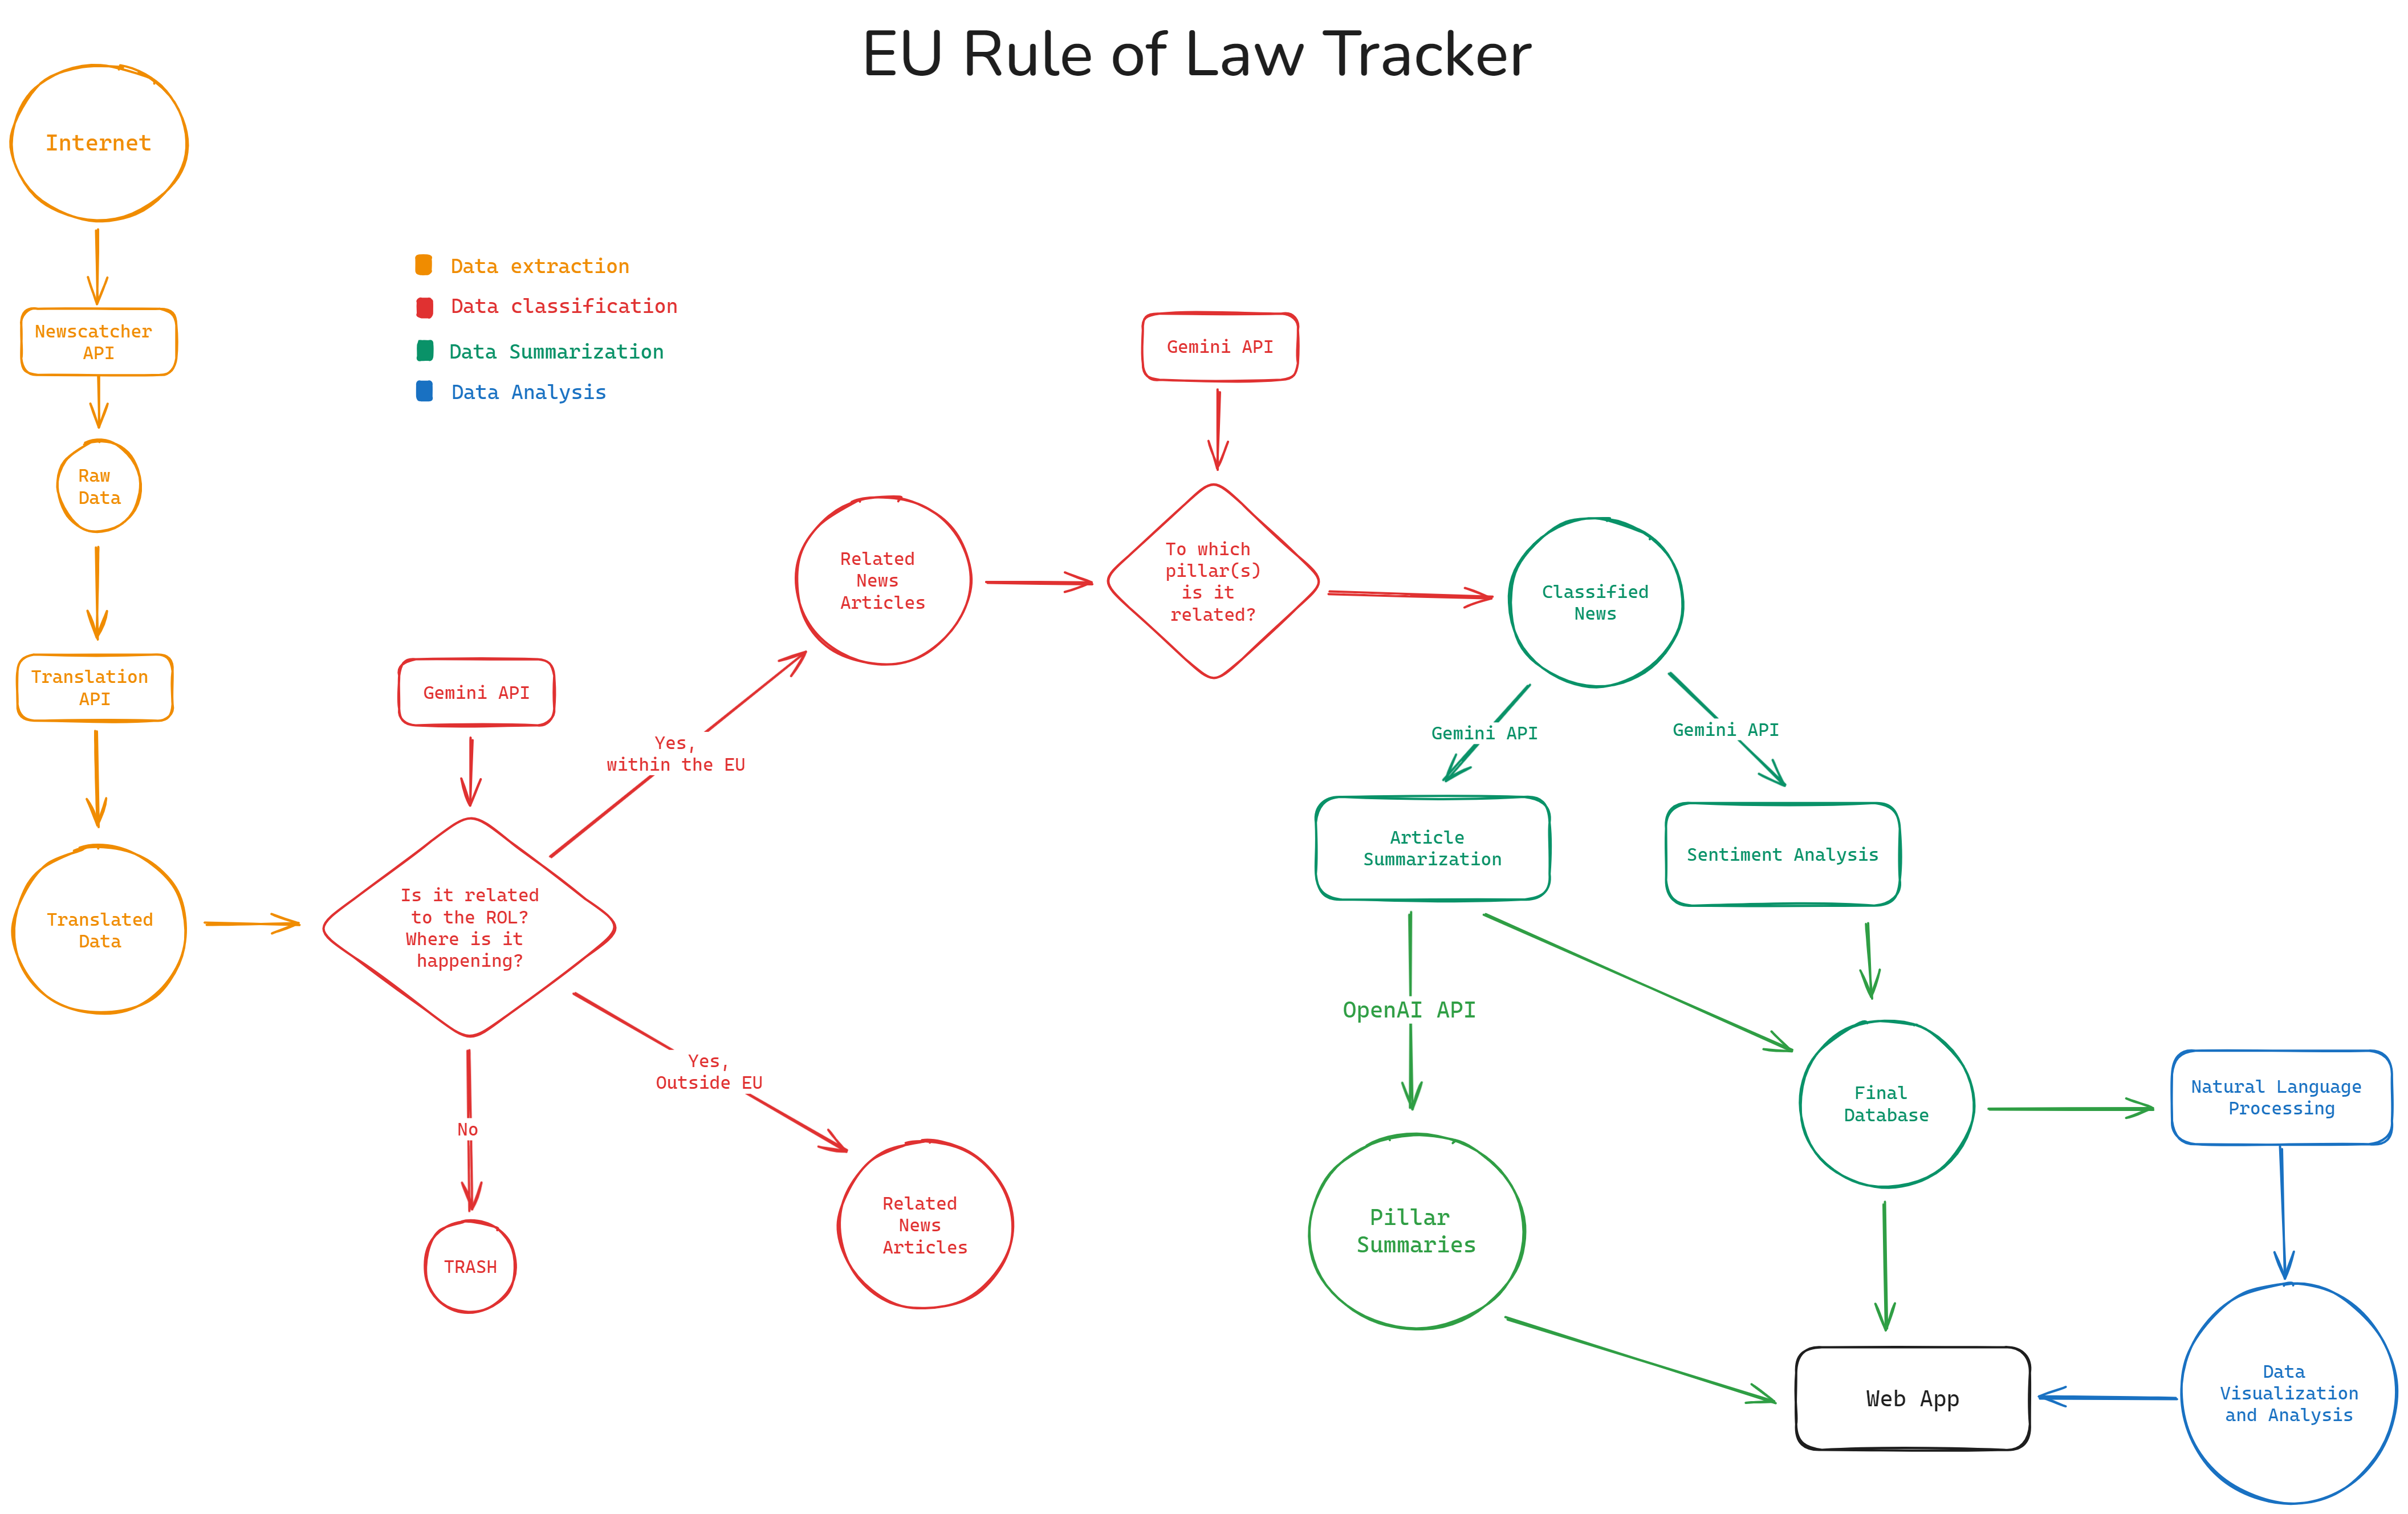
\includegraphics[keepaspectratio]{images/Massive-News-Country-Reports.png}}

}

\end{figure}%

\section[Conceptual Framework]{\texorpdfstring{Conceptual
Framework\sidenote{\footnotesize The concepts outlined in this documents are largely
  based on a preliminary version of the \emph{European Union Subnational
  Indicators: Conceptual and Measurement Framework} document developed
  by The World Justice Project. For more information please consult the
  document here.}}{Conceptual Framework}}\label{conceptual-framework1}

\subsection{Macro-concepts}\label{macro-concepts}

The term Rule of Law refers to a system in which law is able to impose
meaningful restraints on the state and individual members of the ruling
elite. It refers to a governance principle in which all persons,
institutions, and entities, public and private, including the State
itself, are accountable to laws that are publicly promulgated, equally
enforced, and independently adjudicated, and which are consistent with
international human rights norms and standards.

We extend this concept further by defining the Rule of Law as a
rules-based system in which the following four universal principles are
upheld. First, the government and its officials and agents are
accountable under the law. Second, the laws are clear, publicized,
stable, and fair, and protect fundamental rights, including the security
of persons and property. Third, the process by which the laws are
enacted, administered, and enforced is accessible, fair, and efficient.
Lastly, access to justice is provided by competent, independent, and
ethical adjudicators, attorneys or representatives, and judicial
officers who are of sufficient number, have adequate resources, and
reflect the makeup of the communities they serve.

Given the previous definitions, we can infer that the Rule of Law is a
multidimensional concept that extends over eight basic pillars: limited
government powers; absence of corruption; order and security;
fundamental rights; open government; effective regulatory enforcement;
access to civil justice; and an effective criminal justice.

From a political science perspective, these factors draw on four basic
ideas related to the relationship between the state and the civil
society: the checks and balances on the government's power, the
effectiveness of the state in performing its basic functions,
participation and collaboration between the state and its citizens, and
absence of arbitrary abuse by the authority.

We define Justice as the ethical, philosophical idea that people are to
be treated impartially, fairly, properly, and reasonably by the law and
by arbiters of the law, that laws are to ensure that no harm befalls
another, and that, where harm is alleged, a remedial action is taken -
both the accuser and the accused receive a morally right consequence
merited by their actions.

Justice also refers more specifically to the set of institutions and
services that allow for the impartial mediation and adjudication of
disputes arising from the violation or conflicting interpretations of
laws, including the enforcement of decisions or agreements reached
through their operation.

Finally, we define Governance as the mechanisms, processes, and
structures through which public institutions operate and make decisions
for the welfare and benefit of their respective communities. This
encompasses the way governments and local authorities are organized, how
policies are formulated and implemented, how resources are allocated and
managed, and how public services are delivered to citizens.

\subsection{Pillars of the rule of
law}\label{pillars-of-the-rule-of-law}

\subsubsection{Constraints on Government
Powers}\label{constraints-on-government-powers}

Measures the extent to which those who govern are bound by law. It
comprises the means, both constitutional and institutional, by which the
powers of the government and its officials and agents are limited and
held accountable under the law. It also includes non-governmental checks
on the government's power, such as a free and independent press.
Additionally, it measures the absence of authoritarianism, which
includes the accountability of the Chief Executive, and its respect for
checks and balances. In more detail, this pillar is related to the
following topics:

\begin{itemize}
\tightlist
\item
  The active and reactive transparency of legislative bodies (senate,
  parliament, assemblies), its ability to impose disciplinary measures
  to government officials, and if there is representation of
  disadvantaged groups, as well as citizen participation. It also
  measures if the opposition can express its opinions and if it
  exercises its functions of overseeing and investigating the
  government.
\item
  The independence of the judiciary, by means of having sufficient
  resources and professional judges, with adequate rights and
  competencies, as well as its ability to impose disciplinary measures
  on government officials.
\item
  The independence and effectiveness of oversight institutions, such as
  the Supreme Audit Institution or comptroller, anticorruption
  authority, human rights institution, the office of the ombudsman, and
  prosecution services, as well as if civil servants are free from
  political pressure, and are effective in implementing public policies.
\item
  Whether elections are free of barriers of entry, intimidation,
  corruption, and criminality, in accordance with the law, with
  equitable access to resources, free from misinformation, secure from
  cyberattacks and with protection of personal. It also measures the
  effectiveness and independence of the electoral authority.
\item
  The effectiveness of non-governmental checks on the government's
  power, such as the media, CSOs, political parties, activists, and
  citizens. It includes their effective exercise of the freedoms of
  assembly, association, opinion, and expression, and the rights to
  petition and civic engagement.
\item
  The accountability of the Chief Executive or the Head of Government,
  and its respect for the constitutional order, the law-making process,
  the outcome and quality of elections, civil liberties, political
  opponents, as well as the independence of the judiciary and oversight
  institutions. It also measures the likelihood of sanctions to
  officials for misconduct.
\item
  Whether members of the legislature, judiciary, elected leaders or
  high-ranking government officials, public sector employees, and police
  officers, who abuse their power are sanctioned for misconduct.
\end{itemize}

\subsubsection{Abscense of Corruption}\label{abscense-of-corruption}

Measures the control of corruption in various forms: bribery in
administrative and political proceedings, graft, embezzlement, fraud,
payroll fraud, asset misappropriation and skimming, nepotism,
favoritism, patronage, illegal campaign financing, electoral fraud and
vote buying. In more detail, this pillar is related to the following
topics:

\begin{itemize}
\tightlist
\item
  The prevalence of bribery in the delivery of public services and
  regulations, as well as in the political process.
\item
  The prevalence of graft by elected officials, public sector employees,
  by awarding contracts without competitive bidding processes, exerting
  influence for their private benefit, and using insider knowledge to
  profit.
\item
  The prevalence of embezzlement or misappropriation of public funds,
  payroll fraud, asset misappropriation and skimming, as well as of
  nepotism, favoritism, and patronage.
\item
  The prevalence of nepotism and favoritism by elected officials, public
  sector employees, judges, and prosecutors. It also measures the
  prevalence of patronage by elected officials.
\item
  The prevalence of corruption in elections, including illegal campaign
  financing, manipulation of elections, and vote buying.
\end{itemize}

\subsubsection{Open Government}\label{open-government}

Measures the openness of government defined by the extent to which a
government shares information, empowers people with tools to hold the
government accountable, and fosters citizen participation in public
policy deliberations while maintaining an open civic space. This factor
measures whether basic laws and information on legal rights are
publicized and evaluates the quality of information published by the
government. In more detail, this pillar is related to the following
topics:

\begin{itemize}
\tightlist
\item
  Whether requests for information from the public to government
  agencies and institutions are granted, and if these requests are
  granted within a reasonable time period, with complete and pertinent
  answers, at a reasonable cost and without having to pay a bribe for
  the information.
\item
  Whether people are aware of their right to information, and whether
  relevant records are accessible to the public upon request.
\item
  The effectiveness of non-governmental checks on the government's
  power, as well as the openness of the civic space and the extent of
  citizen participation. It includes the effective exercise of the
  freedoms of assembly, association, opinion, and expression, and the
  rights to petition and civic engagement.
\end{itemize}

\subsubsection{Fundamental Rights}\label{fundamental-rights}

This pillar recognizes that a system of positive law that fails to
respect core human rights established under international law is at best
``rule by law,'' and does not deserve to be called a rule of law system.
This aspect focuses on rights that are firmly established under the
Charter of Fundamental Rights of the European Union, but only includes a
relatively small number of rights which are most closely related to rule
of law concerns. In more detail, this pillar is related to the following
topics:

\begin{itemize}
\tightlist
\item
  The protection of rights related to dignity, including the prohibition
  of torture, slavery and forced labor.\\
\item
  The protection of rights related to freedom, including freedom of
  thought, conscience, religion, peaceful assembly, association,
  opinion, and expression, as well as the right to property and to
  asylum.
\item
  Whether civil society organizations are free to comment on government
  policies, without fear of retaliation. In addition, it also measures
  if quarantines and lockdowns are applied proportionately, not
  discriminatory, with limited duration and in accordance with the law.
\item
  Whether independent media, civil society organizations, members of the
  opposition, opposing factions of the governing party, activists,
  whistleblowers, and individuals are free to report and comment on
  government policies, without fear of retaliation.
\item
  The extent to which the media publish credible fact-checked
  information, and if its editorial content is independent from
  political influences, as well as if it can conduct investigations and
  expose cases of corruption without facing surveillance, harassment,
  threats, legal actions, or administrative sanctions.
\item
  The extent to which the government allows the formation or operation
  of CSOs, and the formation or operation of opposition parties.
\item
  Whether the government respects the property rights of people and
  corporations, refrains from the illegal seizure of private property,
  and provides adequate reasons and compensation when property is
  legally expropriated. It also measures if the process for transferring
  a property is simple and quick. In addition, it measures if foreign
  investors receive fair and equitable treatment from the government,
  and the effective enforcement of anti-squatting laws and intellectual
  property rights.
\item
  Whether the government respects the right to asylum and refugees can
  move freely within the host country, have access to legal work and
  state services such as education, accommodation, meals, healthcare,
  and cash benefits, as well as legal documentation and economic
  opportunities.
\item
  The protection of rights related to equality, including equality
  before the law, and absence of discrimination based on socio-economic
  status, gender, ethnicity, religion, national origin, sexual
  orientation, or gender identity.
\item
  The protection of rights related to solidarity, including labor rights
  such as workers' right to information, consultation, collective
  bargaining, access to placement services, and protection in the event
  of unjustified dismissal, as well as the prohibition of child labor.
\item
  The protection of rights related to citizens´ rights, including
  political rights such as the right to vote and to stand as a candidate
  at European Parliament and municipal elections, to information,
  petition, movement, and of residence.
\item
  The protection of rights related to justice, including the right to
  effective remedy and to a fair trial, presumption of innocence, and to
  defense, as well as rights of the accused including principles of
  legality and proportionality of criminal offenses and penalties, and
  the right not to be tried or punished twice.
\end{itemize}

\subsubsection{Security}\label{security}

Measures the assurance of the security of persons and property. Security
is one of the defining aspects of any rule of law society and is a
fundamental function of the state. It is also a precondition for the
realization of the rights and freedoms that the rule of law seeks to
advance. We are excluding armed conflict from this pillar. In more
detail, this pillar is related to the following topics:

\begin{itemize}
\tightlist
\item
  The extent to which people feel safe and secure in their city, town,
  or village, and in their neighborhood.
\item
  The extent to which the State is able to keep crime and violence to
  minimum levels.
\end{itemize}

\subsubsection{Regulatory Enforcement and Enabling Business
Environment}\label{regulatory-enforcement-and-enabling-business-environment}

Measures the extent to which regulations are fairly and effectively
implemented and enforced. Regulations, both legal and administrative,
structure behaviors within and outside of the government. This factor
does not assess which activities a government chooses to regulate, nor
does it consider how much regulation of a particular activity is
appropriate. Rather, it examines how regulations are implemented and
enforced. In more detail, this pillar is related to the following
topics:

\begin{itemize}
\tightlist
\item
  The extent to which the legal framework for businesses is clear,
  accessible, and predictable, as well as the respect for property
  rights.
\item
  Whether the government respects the property rights of people and
  corporations, refrains from the illegal seizure of private property,
  and provides adequate reasons and compensation when property is
  legally expropriated. In addition, it measures if foreign investors
  receive fair and equitable treatment from the government, and the
  effective enforcement of anti-squatting laws and intellectual property
  rights.
\item
  Whether the process for transferring a property is simple and quick.
\item
  The extent to which the government audits and inspections are
  conducted in accordance with the law and are free of corruption; if
  complaint mechanisms are simple, accessible, and cost-effective, and
  if regulation authorities are impartial, and if they sanction
  violations.
\item
  Whether environmental and labor regulation authorities sanction
  violations, such as occupational safety and business license or zoning
  violations.
\end{itemize}

\subsubsection{Civil Justice}\label{civil-justice}

Measures whether ordinary people can resolve their grievances through
formal institutions of justice in a peaceful and effective manner, as
well as in accordance with generally accepted social norms rather than
resorting to violence or self-help. Access to civil justice requires
that the system be accessible, affordable, effective, impartial, and
culturally competent. In more detail, this pillar is related to the
following topics:

\begin{itemize}
\tightlist
\item
  Whether justice institutions help prevent legal and justice needs. It
  also measures whether authorities tolerate illegal activities such as
  squatting, street vending or informal labor arrangements.
\item
  Whether people are aware of their rights, formal justice, and
  alternative justice mechanisms, and know where to get information and
  advice when facing a legal problem.
\item
  Whether can access and afford legal advice and representation; and can
  access the court system without incurring unreasonable fees.
\item
  Whether the civil justice system is impartial and free of
  discrimination, corruption and undue influence from the government and
  private interests.
\item
  The effectiveness and timeliness of the enforcement of civil justice
  decisions and judgments in practice.
\item
  Whether alternative dispute resolution mechanisms (ADRs) are
  available, accessible, affordable, impartial, timely, effective,
  enforceable, and free of corruption and undue influence from the
  government and private interests.
\end{itemize}

\subsubsection{Criminal Justice}\label{criminal-justice}

Evaluates a country's criminal justice system. An effective criminal
justice system is a key aspect of the rule of law, as it constitutes the
conventional mechanism to redress grievances and bring action against
individuals for offenses against society. An assessment of the delivery
of criminal justice should take into consideration the entire system,
including the police, lawyers, prosecutors, judges, and prison officers.
In more detail, this pillar is related to the following topics:

\begin{itemize}
\tightlist
\item
  Whether criminal investigations are effective, timely, impartial, and
  free of corruption and undue influence from criminal organizations and
  political and private interests.
\item
  The effectiveness of prosecutors in investigating crimes, and if
  pre-trial proceedings are timely, outcome-oriented, impartial, and
  free of corruption and undue influence from political and private
  interests.
\item
  Whether trials are timely, outcome-oriented, impartial, and free of
  corruption and undue influence from political and private interests.
\item
  Whether alternative dispute resolution mechanisms (ADRs) are
  available, accessible, affordable, impartial, timely, effective,
  enforceable, and free of corruption and undue influence from the
  government and private interests.
\item
  Whether victim's rights are effectively guaranteed, including
  treatment with respect, absence of discrimination, timely and
  sufficient information, and protection.
\item
  Whether the basic rights of criminal suspects are respected, including
  the presumption of innocence and the freedom from arbitrary arrest and
  unreasonable pre-trial detention. It also measures whether criminal
  suspects are able to access and challenge evidence used against them,
  whether they are subject to abusive treatment, and whether they are
  provided with adequate legal assistance. In addition, it measures
  whether the basic rights of prisoners are respected once they have
  been convicted of a crime.
\item
  Whether the prison system guarantees conditions of safety and order
  and respects the rights of people deprived of their liberty. It also
  measures the absence of corruption and the effectiveness of the prison
  system in reducing recidivism.
\end{itemize}

\section{Extraction and Translation}\label{extraction-and-translation}

The first step in designing the \emph{EU Rule of Law Tracker} was to
identify, gather, and compile the information that would serve as the
primary input for the tracker. Several inputs such as official records,
social media, academic research, and think tanks publications were
considered. Several sources, including official records, social media,
academic research, and think tank publications, were considered. After a
careful review, it was decided to use news articles for the pilot
version of the tracker due to several advantages.

First, multiple data archives offer harmonized databases for a wide
range of newspapers from around the world, often accessible via
Application Programming Interfaces (APIs). These databases are
frequently updated, providing near real-time access to the latest
events. In contrast, alternative data sources, such as academic
publications and official records, generally have longer research,
editorial, and publishing times, resulting in less timely information
compared to most newspapers.

Second, news articles come from a wide variety of media outlets. Each
with its own editorial line and cultural context. Given the political
nature of the events that are usually associated to the Rule of Law, it
is of highly importance to ensure the diversity of viewpoints so our
final outcome have a more nuanced understanding of how the events are
shaping the political and social environment across different countries.

Third, newspapers create a historical record of events that can be
tracked over time. They also offer a resource that is easily accessible
to the general public. Moreover, competition for readership among
newspapers often drives journalists to provide additional research,
background information, and context, enhancing the quality of reporting.

On the other hand, relying on news articles as the primary data source
for tracking democracy and rule of law events also presents some
drawbacks. The most significant challenges are the risks of media bias,
subjectivity, and sensationalism. Additionally, the quality and
consistency of data can vary significantly between sources, posing risks
related to misinformation, lack of depth, and disparities in regional
coverage.

To mitigate these potential risks, we limited our selection to 211
newspapers. The list was curated based on five key criteria to ensure
balanced and reliable coverage:(i) editorial influence, (ii) historical
significance, (iii) audience reach, (iv) diversity of editorial
perspectives, and (v) regional representation. Additionally, the
newspapers were categorized to identify \emph{priority} and
\emph{high-priority} sources within each of the 27 member states of the
European Union. Of the 211 sources, 153 were designated as priority,
while 84 were labeled as high-priority. The full list of data sources
can be found in Section~\ref{sec-sources}. Due to limited resources
during the news extraction phase, only high-priority sources were used
in the pilot version of the tracker.

Having identified and delimited the pool of data sources for the study,
we needed a way to access and download the news articles for the
tracker. For this purpose, we made use of a news API service called
\href{https://www.newscatcherapi.com/}{Newscatcher}. A news API is a
programming interface that allows users to access and retrieve news
articles from a wide variety of sources. By using
\href{https://developer.mozilla.org/en-US/docs/Web/HTTP/Methods}{HTTP
calls}, we are able to access the data archive compiled by the company
and retrieve news articles based on some query parameters. The
Newscatcher API allows to search news based on dates, languages,
sources, URL, among other optional parameters. Additionally, their data
archive tracks all of our 84 high-priority newspapers.

However, it is not possible to directly query for news articles solely
related to our definition of the rule of law. As a workaround, we
developed queries using specific keywords associated with our definition
of the rule of law and its dimensions, as well as broader concepts like
justice and governance. Our strategy focused on performing a \emph{wide
search} rather than a \emph{narrow search}. In other words, we
intentionally used broad, general keywords to ensure that our results
included a wide range of articles, even at the risk of retrieving some
unrelated content. This approach was chosen to avoid excluding
potentially relevant articles. The process of refining the search
results through text classification using Large Language Models (LLMs)
is covered in detail in Section~\ref{sec-class}.

For the extraction, we defined a total of 137 keywords. These keywords
are divided into 123 language-based keywords and 14 country-based
institutional keywords. The language-based keywords encompass common
nouns that are shared across countries that shared the same official
language. For example ``\emph{Kongress}'' is the German word for
Congress and it can be equally used in news articles from newspapers in
Germany as well by newspapers in Austria. However, even when these two
countries share the same language, they might refer to some institutions
in different ways. For example, ``\emph{Verfassungsgerichtshof}'' is how
Austrian newspapers might refer to the Constitutional Court, while
German newspapers might refer to it as
``\emph{Bundesverfassungsgericht}''.

Depending on the language of publication of each targeted newspaper, we
will use a combination of language- and country-based keywords (see
Figure~\ref{fig-keywords}). For example, the newspaper ``\emph{De
Standaard}'' in Belgium publishes news in Dutch. Therefore, we will use
the 123 language-based keywords in Dutch (also used in some newspapers
from the Netherlands), as well as the 14 Belgium institutions names in
Dutch (unique for Belgium). On the other hand, the Belgium newspaper
``\emph{Le Soir}'' publishes their news in French. As a result, we use
the 123 french keywords (also used for Newspapers in France), as well as
the 14 Belgium institution names in French (unique for Belgium
newspapers). The definition of keywords was made in English and then
manually translated to the other 22 languages used by the rest of the
targeted newspapers.\sidenote{\footnotesize The translation of these keywords involved
  a combination of desk research, translation engines, and native
  speaker consultations when possible.} The full list of keywords can be
consulted in Section~\ref{sec-keys}.

\begin{figure}

\caption{\label{fig-keywords}Keywords used for extraction}

\centering{

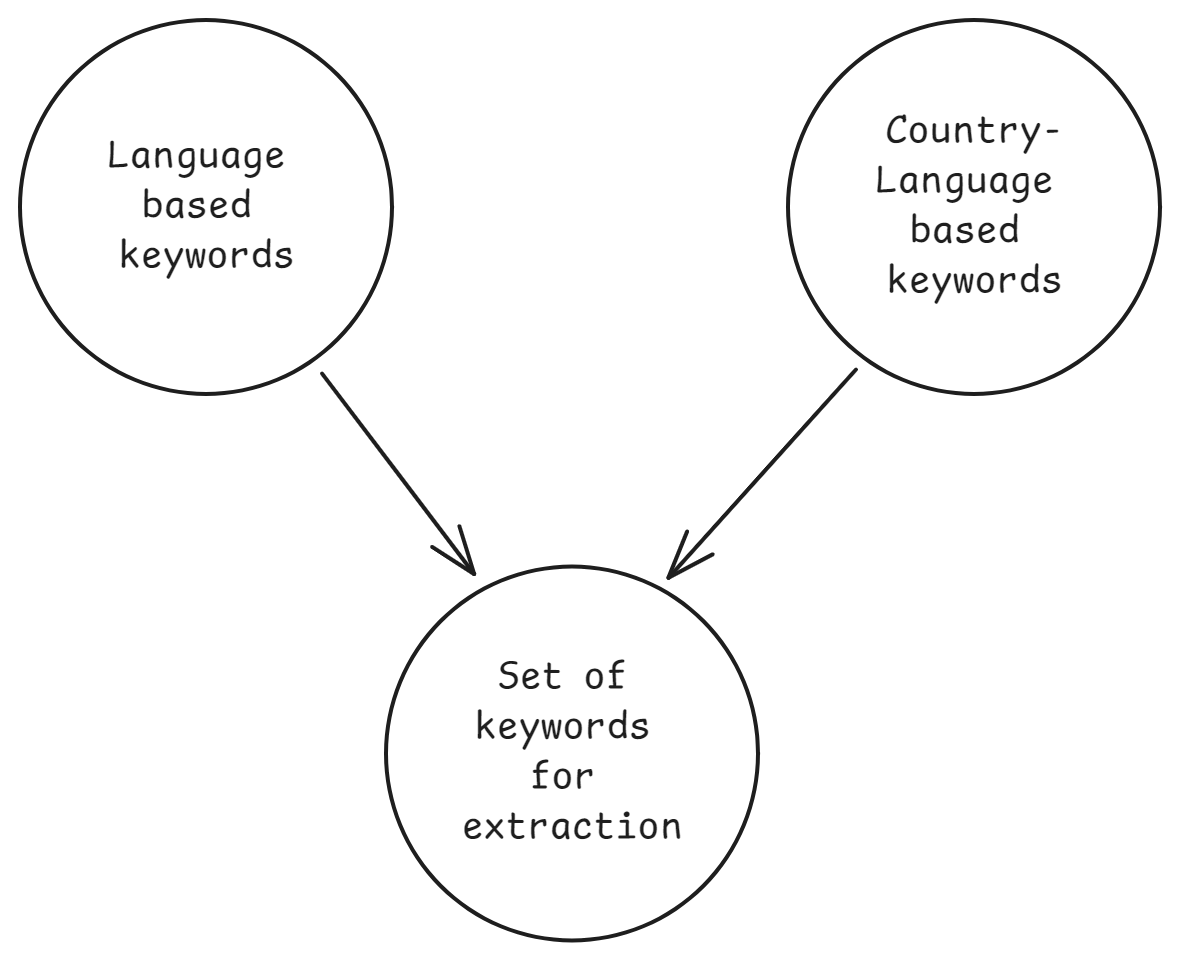
\includegraphics[width=0.75\linewidth,height=\textheight,keepaspectratio]{images/keywords.png}

}

\end{figure}%

Due to quota limitations at the time of the extraction,\sidenote{\footnotesize At the
  time of the extraction, Newscatcher was transitioning from version 2
  to version 3 of their API. While the v2 version of their API was able
  to go further back to even 2 years in the past, the v3 version was
  only able to capture news articles from the past 3 months. Due to
  technology transitions, we had a limit of 20,000 calls for their
  version 2, which is equivalent to a total of 800,000 news articles} a
time range of eight months was targeted for most countries with a few
exceptions (see Table~\ref{tbl-extraction}). A total of 904,944 news
articles were gathered from the Newscatcher data archive. The data
consisted of tabular data in JSON format. The response object returned
by the API contained some information from the news articles such as the
published date, title, content, language, URL, and if the article was
coming from an opinion column or a regular section of the newspaper. The
code used for the extraction phase can be found in the
\href{https://ctoruno.github.io/eu-rol-tracker/notebooks/0_EU_news_gathering_1-preview.html}{Extraction
notebook} in the supplementary materials to this manuscript.

\begin{longtable}[]{@{}lll@{}}

\caption{\label{tbl-extraction}Total news extracted per country}

\tabularnewline

\caption{}\label{T_1f17c}\tabularnewline
\toprule\noalign{}
Country & Total News Extracted & Date Range \\
\midrule\noalign{}
\endfirsthead
\toprule\noalign{}
Country & Total News Extracted & Date Range \\
\midrule\noalign{}
\endhead
\bottomrule\noalign{}
\endlastfoot
Austria & 46,145 & Mar 06, 2023 - Mar 07, 2024 \\
Belgium & 21,287 & Jun 07, 2023 - Mar 07, 2024 \\
Bulgaria & 38,118 & Jul 07, 2023 - Mar 07, 2024 \\
Croatia & 37,068 & Jul 07, 2023 - Mar 07, 2024 \\
Cyprus & 34,955 & Jul 07, 2023 - Mar 08, 2024 \\
Czechia & 41,415 & Jul 07, 2023 - Mar 08, 2024 \\
Denmark & 11,312 & Aug 07, 2023 - Mar 07, 2024 \\
Estonia & 12,370 & Aug 08, 2023 - Mar 07, 2024 \\
Finland & 6,647 & Aug 08, 2023 - Mar 07, 2024 \\
France & 64,527 & Aug 07, 2023 - Mar 07, 2024 \\
Germany & 45,321 & Jan 08, 2024 - Mar 07, 2024 \\
Greece & 49,504 & Aug 08, 2023 - Mar 07, 2024 \\
Hungary & 18,111 & Aug 08, 2023 - Mar 07, 2024 \\
Ireland & 48,409 & Aug 08, 2023 - Mar 07, 2024 \\
Italy & 93,858 & Aug 08, 2023 - Mar 07, 2024 \\
Latvia & 5,487 & Aug 09, 2023 - Mar 07, 2024 \\
Lithuania & 14,396 & Aug 08, 2023 - Mar 07, 2024 \\
Luxembourg & 7,894 & Aug 08, 2023 - Mar 07, 2024 \\
Malta & 10,842 & Aug 08, 2023 - Mar 07, 2024 \\
Netherlands & 23,935 & Aug 08, 2023 - Mar 07, 2024 \\
Poland & 21,434 & Aug 08, 2023 - Mar 07, 2024 \\
Portugal & 29,624 & Aug 08, 2023 - Mar 07, 2024 \\
Romania & 33,264 & Aug 08, 2023 - Mar 07, 2024 \\
Slovakia & 34,874 & Aug 08, 2023 - Mar 07, 2024 \\
Slovenia & 10,211 & Aug 08, 2023 - Mar 07, 2024 \\
Spain & 112,820 & Aug 08, 2023 - Mar 07, 2024 \\
Sweden & 6,417 & Jan 08, 2024 - Mar 07, 2024 \\
Total & 880,245 & \\

\end{longtable}

\textsubscript{Source:
\href{https://ctoruno.github.io/eu-rol-tracker/notebooks/tables-preview.html\#cell-tbl-extraction}{Tables}}

The titles and content of the news articles were returned in their
original publication languages, resulting in a diverse collection of
information in 23 different languages: Bulgarian, Croatian, Czech,
Danish, Dutch, English, Estonian, Finnish, French, German, Greek,
Hungarian, Italian, Latvian, Lithuanian, Maltese, Polish, Portuguese,
Romanian, Slovak, Slovene, Spanish, and Swedish. While this linguistic
diversity highlights the cultural richness of the region, it also
presents challenges for accurate classification and text analysis.

The LLMs used in this project are multilingual models, but their
accuracy in text classification can vary across languages (Unanue et
al., 2023). To ensure consistency during the classification process and
to facilitate the use of NLP techniques in the data analysis phase, we
decided to translate all the data into a single language. Since most
LLMs are primarily trained on English data, we chose English as the
target language for translation. To guarantee the highest quality, we
used the Google Translation API to translate all of our text data. The
code used for the translation phase can be found in the
\href{https://ctoruno.github.io/eu-rol-tracker/notebooks/1_EU_news_translation_1-preview.html}{Translation
notebook} in the supplementary materials to this manuscript.

A total of 808,429 news articles, equivalent to 93.9\% of the total
number of articles extracted, were successfully translated. This lost of
information was due to several reasons such as API connection failures,
news articles with empty content, corrupted text data, unidentified
source language, among other reasons, unusually long text, among other
reasons. Column 4 in Table~\ref{tbl-translation} contains information on
the success rate per country during the translation process.

\begin{longtable}[]{@{}llll@{}}

\caption{\label{tbl-translation}Translation Process (Rate of Success)}

\tabularnewline

\caption{}\label{T_542c5}\tabularnewline
\toprule\noalign{}
Country & Extracted News (n) & Translated News (n) & Translated News
(\%) \\
\midrule\noalign{}
\endfirsthead
\toprule\noalign{}
Country & Extracted News (n) & Translated News (n) & Translated News
(\%) \\
\midrule\noalign{}
\endhead
\bottomrule\noalign{}
\endlastfoot
Austria & 46,145 & 44,181 & 95.7 \\
Belgium & 21,287 & 19,846 & 93.2 \\
Bulgaria & 38,118 & 33,070 & 86.8 \\
Croatia & 37,068 & 36,595 & 98.7 \\
Cyprus & 34,955 & 33,772 & 96.6 \\
Czechia & 41,415 & 40,620 & 98.1 \\
Denmark & 11,312 & 10,761 & 95.1 \\
Estonia & 12,370 & 11,334 & 91.6 \\
Finland & 6,647 & 6,399 & 96.3 \\
France & 64,527 & 62,900 & 97.5 \\
Germany & 45,321 & 40,444 & 89.2 \\
Greece & 49,504 & 47,182 & 95.3 \\
Hungary & 18,111 & 17,965 & 99.2 \\
Ireland & 48,409 & 48,409 & 100.0 \\
Italy & 93,858 & 82,885 & 88.3 \\
Latvia & 5,487 & 5,467 & 99.6 \\
Lithuania & 14,396 & 13,287 & 92.3 \\
Luxembourg & 7,894 & 7,636 & 96.7 \\
Malta & 10,842 & 10,556 & 97.4 \\
Netherlands & 23,935 & 22,642 & 94.6 \\
Poland & 21,434 & 17,490 & 81.6 \\
Portugal & 29,624 & 29,416 & 99.3 \\
Romania & 33,264 & 32,234 & 96.9 \\
Slovakia & 34,874 & 28,973 & 83.1 \\
Slovenia & 10,211 & 9,818 & 96.2 \\
Spain & 112,820 & 88,324 & 78.3 \\
Sweden & 6,417 & 6,223 & 97.0 \\
European Union & 880,245 & 808,429 & 93.9 \\

\end{longtable}

\textsubscript{Source:
\href{https://ctoruno.github.io/eu-rol-tracker/notebooks/tables-preview.html\#cell-tbl-translation}{Tables}}

\section{Classification}\label{sec-class}

The extraction and translation phase provided us with a diverse database
of news articles from a wide range of sources. However, as previously
mentioned, there is a significant risk of including articles that
narrate events unrelated to our definitions of Rule of Law, Justice, and
Governance. To meet the project's objectives, it is crucial that the
system can not only differentiate between articles that are relevant to
our macro-concepts and those that are not, but also accurately classify
the relevant articles according to the specific pillars of the rule of
law that they are related to. In order to achieve this, we made use of
the text classification capabilities of Large Language Models such as
\href{https://platform.openai.com/docs/concepts}{GPT} and
\href{https://ai.google.dev/gemini-api/docs?_gl=1*1ixp628*_ga*NzAxMDUzNTUyLjE3MDQ0NTQ0NzA.*_ga_P1DBVKWT6V*MTcyNTkwNDYyMi40OC4wLjE3MjU5MDQ2MjIuNjAuMC41MjU1MDg0ODg.}{Gemini}.\sidenote{\footnotesize GPT
  refers to a family of models developed by OpenAI, while Gemini refers
  to a family of models developed by Google. During the pilot phase of
  this study, we tested the \emph{GPT-4-Turbo} and the \emph{Gemini-1.5}
  models, respectively.}

We divided the classification phase into two stages. In the first stage,
the system aims to categorize news articles based on whether they are
related to our concepts of Rule of Law, Justice, and Governance, or not.
Additionally, the system will identify the location where the events
described in the article are taking place. During this stage, the total
number of news articles that were successfully translated are passed to
the model.

In the second stage, the system will further classify the relevant
articles according to which specific pillars of the rule of law the
events are related to. This stage focuses exclusively on articles that
were previously classified as related to our macro-concepts and that
describe events occurring within one of the 27 member states of the
European Union.

\subsection{Prompt definition}\label{prompt-definition}

In both stages, we defined two prompt templates to pass to the LLM: a
system context and the instructions. The system context is a type of
prompt used to set the context or guide the behavior of the model during
a conversation. In our specific case, the system context was used to
establish the role of the model as an assistant, provide general
instructions and some background information of the purpose of the
tasks. The instruction template contained the conceptual framework, the
full text of the article, some key point to take into account, as well
as specific instructions on how to structure the answers (JSON format).
The full text of the prompts used can be found in the
\href{https://ctoruno.github.io/eu-rol-tracker/notebooks/prompts_classification-preview.html}{Prompt
templates: Text Classification notebook} in the supplementary materials
to this manuscript.

These prompts were the results of a dynamic and iterative process of
\href{https://platform.openai.com/docs/guides/prompt-engineering/strategy-write-clear-instructions}{prompt
engineering}. More specifically, we randomly selected a batch 100 news
articles and then we proceeded to classify them using the GPT and Gemini
models along with a project-specific
\href{https://www.langchain.com/}{LangChain workflow}.\sidenote{\footnotesize LangChain
  is an open-source framework that facilitates the integration of
  generative AI models into your own framework. You can see it as a
  toolkit that covers and provide easy and fast solutions to many of the
  usual tasks that programmers face when dealing with language models.}
Once that the models finished classifying the testing batch, two experts
were consulted to evaluate and provide feedback on the accuracy of the
classification. The experts were contextualized on the purpose of the
exercise in order to get a correct assessment on how well the models
were classifying the news articles and how can it be improved through
clear instructions. Once that their feedback was received, we proceeded
to adjust the prompts and repeat the exercise once again. This exercise
was repeated four times until reaching a point in which further
instructions were reducing the accuracy of the classification due to an
increase in the complexity of the prompt.

In all rounds of testing, the \emph{GPT-4-Turbo} model exhibited higher
accuracy and precision than the \emph{Gemini-1.0-Pro} model. However,
both models exhibited a good performance when compared to human
classification (see Section~\ref{sec-accuracy}). Due to costs restraints
for this project, the classification stage for the full sample of news
article was performed using only the \emph{Gemini-1.0-Pro}
model.\sidenote{\footnotesize The Gemini model was introduced to the market in
  December 2023. Sending calls to the model through the Google AI API
  was free as long as the overall use remained under 60 requests per
  minute (RPM). This policy was in place until May 2024.}

\subsection{First stage: Broad
classification}\label{first-stage-broad-classification}

For the first stage, we used an 85-word system context that remained
fixed in every call made to the LLM, along with a 583-word instruction
prompt template.\sidenote{\footnotesize The final instruction prompt would usually be
  longer due to the inclusion of the title and full content of the news
  article.} During this stage, the main objective is to reduce the
universe of news articles to be classified. The process was outlined
this way to reduce the monetary and computing costs of passing more
detailed instructions over the whole universe of news
articles.\sidenote{\footnotesize Monetary and computational costs of using Large
  Language Models are based on token counts. By breaking the process in
  two stages, we were able to reduce the total token count
  (instructions-only) to 99 million tokens in comparison to an
  hypothetical scenario of 2,459 million tokens (instructions-only) if
  we had passed the detailed instructions to all 808,429 news articles
  from the beginning.} Therefore, the instructions prompt used in this
stage contains very general definitions of our macro-concepts and the
main outcome is a binary answer classifying the articles as related or
not to our conceptual framework.

Out of the 808,429 articles that were passed to the
\emph{Gemini-1.0-Pro} model, an average of 27.8\% were categorized as
related to our definitions of rule of law, justice, and governance.
However, this proportion varied significantly, reaching as high as
43.6\% in Romania and dropping to just 8\% in Ireland (column {[}2{]},
Table~\ref{tbl-classstage1}). However, articles from a newspaper in
France, for example, might narrate events occurring in other parts of
the world. When focusing only on those articles narrating events that
happened within the same country in which the newspaper is based, an
average of 18.7\% were classified by the model as related to our
macro-concepts. Similarly, this proportion can reach as high as 33.7\%
in Poland and as low as 5.5\% in Ireland (column {[}3{]},
Table~\ref{tbl-classstage1}).

During this stage, a small percentage of news articles could not be
classified because the prompt sent to the model was blocked by the API.
Like other large language models, Gemini employs various techniques to
filter and block harmful or inappropriate prompts. These measures are
designed to ensure that the model generates safe, helpful, and unbiased
content. Even after reducing the security settings to the minimum, some
prompts were still blocked due to their content. On average, less than
1\% of the total news articles were unable to be classified for this
reason (column {[}5{]}, Table~\ref{tbl-classstage1}).

A total of 148,124 news articles were passed to the
\emph{Gemini-1.0-Pro} model for further classification.

\begin{longtable}[]{@{}lllll@{}}

\caption{\label{tbl-classstage1}Broad classification results}

\tabularnewline

\caption{}\label{T_9487f}\tabularnewline
\toprule\noalign{}
Country & Related (\%) & Related - Within (\%) & Related - Within (n) &
Unclassified (\%) \\
\midrule\noalign{}
\endfirsthead
\toprule\noalign{}
Country & Related (\%) & Related - Within (\%) & Related - Within (n) &
Unclassified (\%) \\
\midrule\noalign{}
\endhead
\bottomrule\noalign{}
\endlastfoot
Austria & 24.9 & 12.7 & 5,590 & 0.5 \\
Belgium & 24.2 & 13.8 & 2,737 & 1.0 \\
Bulgaria & 35.1 & 24.4 & 8,071 & 0.3 \\
Croatia & 28.8 & 17.6 & 6,431 & 0.8 \\
Cyprus & 29.1 & 19.9 & 6,716 & 0.3 \\
Czechia & 21.8 & 17.5 & 7,114 & 1.3 \\
Denmark & 30.6 & 17.6 & 1,897 & 0.9 \\
Estonia & 22.5 & 14.1 & 1,599 & 0.3 \\
Finland & 32.8 & 23.5 & 1,501 & 0.8 \\
France & 26.5 & 15.8 & 9,955 & 0.7 \\
Germany & 29.4 & 23.0 & 9,292 & 0.8 \\
Greece & 26.6 & 17.1 & 8,027 & 1.2 \\
Hungary & 25.8 & 15.4 & 2,768 & 0.8 \\
Ireland & 8.0 & 5.5 & 2,676 & 0.2 \\
Italy & 29.1 & 24.1 & 18,800 & 0.8 \\
Latvia & 15.1 & 11.6 & 636 & 0.6 \\
Lithuania & 31.5 & 24.6 & 3,272 & 0.7 \\
Luxembourg & 26.7 & 14.7 & 1,119 & 0.5 \\
Malta & 37.6 & 30.4 & 3,205 & 0.4 \\
Netherlands & 24.8 & 14.2 & 3,223 & 0.6 \\
Poland & 40.7 & 33.7 & 5,902 & 0.8 \\
Portugal & 23.2 & 14.8 & 4,217 & 0.3 \\
Romania & 43.6 & 27.2 & 8,765 & 1.0 \\
Slovakia & 26.8 & 17.9 & 5,172 & 0.4 \\
Slovenia & 30.7 & 18.2 & 1,786 & 0.7 \\
Spain & 27.7 & 18.9 & 16,685 & 1.0 \\
Sweden & 26.7 & 15.6 & 968 & 2.5 \\
European Union & 27.8 & 18.7 & 148,124 & 0.8 \\

\end{longtable}

\textsubscript{Source:
\href{https://ctoruno.github.io/eu-rol-tracker/notebooks/tables-preview.html\#cell-tbl-classstage1}{Tables}}

\subsection{Second stage: Pillar
classification}\label{second-stage-pillar-classification}

For the second stage, we used a fixed 114-word system context in every
call to the LLM, along with a 2,928-word instruction prompt template
that provided detailed definitions of each pillar. The primary objective
during this stage was for the system to classify articles based on which
specific pillar of the Rule of Law the events described in the text were
related to. However, due to the close relationship and theoretical
overlap between the pillars in our conceptual framework, an article
could be associated with multiple pillars. As a result, the main output
of this stage was a vector of eight binary values, where each value
would be set to one if the events in the article were related to a
specific pillar, and zero otherwise.

Nevertheless, the overlapping nature of the pillars meant that some
events could be strongly or mildly correlated with several pillars. If
left unchecked, this overlap could lead to an ``\emph{overlabeling}''
scenario where articles would be classified as relevant to nearly all
dimensions of the rule of law. To mitigate this, the instructions passed
to the LLM were designed so the model would focus in providing a ranking
score on how strongly a news article is correlated with each pillar on a
scale from 0 to 10, with 0 indicating no relevance and 10 indicating a
strong correlation. This vector is then transformed into a series of
binary values using the following rule:

Let \(\mathbf{s} = (s_1, s_2, \dots, s_8)\) represent the score vector
for a news article across the eight pillars, where \(s_i \in [0, 10]\)
represents the score for pillar (i).

The transformation into binary values is defined by a threshold (\(T\)),
such that the binary classification for each pillar is given by:

\[
b_i =
\begin{cases}
1 & \text{if } s_i \geq T \\
0 & \text{if } s_i < T
\end{cases}
\]

where (\(b_i\)) is the binary value indicating whether the article is
related to pillar (i). If (\(s_i \geq T\)), the article is classified as
related to pillar (i) (i.e., (\(b_i = 1\))); otherwise, it is unrelated
(i.e., (\(b_i = 0\))).

Table~\ref{tbl-classstage2} displays the results of the second stage.
More specifically, the percentage of news articles associated to each of
the eight predefined dimensions of the rule of law. On average, the
system found a strong presence of news articles related to
\emph{Constraints on Government Powers} (Pillar 1, 20.9\%),
\emph{Criminal Justice} (Pillar 8, 17.1\%), and \emph{Fundamental
Rights} (Pillar 4, 16.7\%). On the other hand, the system found very few
news articles related to \emph{Open Government} (Pillar 3, 2.9\%) and
\emph{Regulatory Enforcement} (Pillar 6, 3.9\%). However, these
percentages present substantial variations when considering the
associations at the country level.

\begin{longtable}[]{@{}lllllllll@{}}

\caption{\label{tbl-classstage2}Pillar classification results (\%)}

\tabularnewline

\caption{}\label{T_259f0}\tabularnewline
\toprule\noalign{}
Country & Pillar 1 & Pillar 2 & Pillar 3 & Pillar 4 & Pillar 5 & Pillar
6 & Pillar 7 & Pillar 8 \\
\midrule\noalign{}
\endfirsthead
\toprule\noalign{}
Country & Pillar 1 & Pillar 2 & Pillar 3 & Pillar 4 & Pillar 5 & Pillar
6 & Pillar 7 & Pillar 8 \\
\midrule\noalign{}
\endhead
\bottomrule\noalign{}
\endlastfoot
Austria & 18.9 & 9.8 & 2.2 & 15.3 & 5.8 & 2.5 & 6.1 & 15.8 \\
Belgium & 13.3 & 9.0 & 1.4 & 12.8 & 5.8 & 1.9 & 6.5 & 17.1 \\
Bulgaria & 27.4 & 16.7 & 3.6 & 17.8 & 8.1 & 5.2 & 9.2 & 21.3 \\
Croatia & 20.6 & 13.0 & 2.3 & 15.6 & 8.1 & 3.0 & 6.5 & 19.8 \\
Cyprus & 22.6 & 13.7 & 3.9 & 16.2 & 7.5 & 6.1 & 7.9 & 15.6 \\
Czechia & 14.7 & 9.1 & 1.7 & 10.8 & 6.6 & 2.7 & 4.6 & 14.6 \\
Denmark & 24.3 & 12.8 & 3.0 & 20.2 & 9.2 & 3.0 & 8.2 & 20.5 \\
Estonia & 16.9 & 8.9 & 2.0 & 11.7 & 4.3 & 3.4 & 5.9 & 13.2 \\
Finland & 24.2 & 12.9 & 1.9 & 20.3 & 10.2 & 3.6 & 8.2 & 22.5 \\
France & 20.5 & 9.7 & 2.3 & 18.5 & 7.1 & 3.1 & 5.6 & 15.3 \\
Germany & 20.9 & 9.5 & 2.1 & 17.7 & 9.2 & 2.5 & 7.0 & 19.4 \\
Greece & 20.2 & 12.1 & 2.6 & 16.7 & 8.6 & 3.9 & 6.3 & 17.4 \\
Hungary & 21.8 & 13.2 & 2.6 & 16.4 & 5.9 & 3.6 & 4.0 & 14.0 \\
Ireland & 18.6 & 9.4 & 2.7 & 16.5 & 7.0 & 3.7 & 8.0 & 16.2 \\
Italy & 17.9 & 12.3 & 2.5 & 17.2 & 8.2 & 4.1 & 7.4 & 18.4 \\
Latvia & 10.4 & 6.1 & 2.0 & 7.5 & 3.1 & 3.3 & 2.1 & 6.2 \\
Lithuania & 22.7 & 14.1 & 2.4 & 15.3 & 6.6 & 4.4 & 7.7 & 20.7 \\
Luxembourg & 16.4 & 8.3 & 3.8 & 15.8 & 6.6 & 3.7 & 5.8 & 13.1 \\
Malta & 30.1 & 19.3 & 7.4 & 24.0 & 6.4 & 9.2 & 13.0 & 21.4 \\
Netherlands & 16.6 & 9.6 & 2.6 & 15.5 & 5.6 & 3.0 & 6.0 & 14.8 \\
Poland & 31.6 & 18.1 & 3.8 & 23.1 & 7.6 & 5.6 & 11.4 & 23.5 \\
Portugal & 18.6 & 9.5 & 3.0 & 13.6 & 3.1 & 3.6 & 5.2 & 10.6 \\
Romania & 28.6 & 23.3 & 4.1 & 22.5 & 9.5 & 7.0 & 8.1 & 25.0 \\
Slovakia & 23.1 & 13.0 & 3.6 & 16.0 & 4.6 & 3.0 & 4.9 & 15.5 \\
Slovenia & 24.4 & 11.9 & 3.1 & 18.4 & 7.4 & 4.3 & 7.4 & 16.4 \\
Spain & 20.6 & 11.0 & 2.6 & 17.3 & 6.3 & 3.3 & 6.1 & 15.8 \\
Sweden & 19.8 & 10.2 & 1.9 & 18.1 & 9.7 & 2.0 & 6.3 & 19.1 \\
European Union & 20.9 & 12.1 & 2.9 & 16.7 & 7.0 & 3.9 & 6.9 & 17.1 \\

\end{longtable}

\textsubscript{Source:
\href{https://ctoruno.github.io/eu-rol-tracker/notebooks/tables-preview.html\#cell-tbl-classstage2}{Tables}}

Percentages across pillars in Table~\ref{tbl-classstage2} do not sum up
to 100 due to three reasons. First, one single article could be
associated to multiple pillars. Second, when given more detailed
information on the rule of law and its different dimensions, some news
articles might have received new scores that would reflect their
disassociation from our theoretical framework. Third, some news articles
were only mildly related to all of the pillars considered in our
conceptual framework.

\subsection{How accurate is the text
classification?}\label{sec-accuracy}

\section{Summarization and Sentiment}\label{summarization-and-sentiment}

\section{Text Insights}\label{text-insights}

\section{Next Steps}\label{next-steps}

\section{Appendix}\label{appendix}

\subsection{List of data sources}\label{sec-sources}

\begin{tcolorbox}[enhanced jigsaw, colframe=quarto-callout-note-color-frame, breakable, leftrule=.75mm, left=2mm, colback=white, title=\textcolor{quarto-callout-note-color}{\faInfo}\hspace{0.5em}{Data sources}, opacityback=0, opacitybacktitle=0.6, toprule=.15mm, bottomtitle=1mm, bottomrule=.15mm, titlerule=0mm, arc=.35mm, rightrule=.15mm, colbacktitle=quarto-callout-note-color!10!white, coltitle=black, toptitle=1mm]

\begin{longtable}[]{@{}
  >{\raggedright\arraybackslash}p{(\linewidth - 16\tabcolsep) * \real{0.0706}}
  >{\raggedright\arraybackslash}p{(\linewidth - 16\tabcolsep) * \real{0.2353}}
  >{\raggedright\arraybackslash}p{(\linewidth - 16\tabcolsep) * \real{0.1588}}
  >{\raggedright\arraybackslash}p{(\linewidth - 16\tabcolsep) * \real{0.0353}}
  >{\raggedright\arraybackslash}p{(\linewidth - 16\tabcolsep) * \real{0.2176}}
  >{\raggedright\arraybackslash}p{(\linewidth - 16\tabcolsep) * \real{0.0647}}
  >{\raggedright\arraybackslash}p{(\linewidth - 16\tabcolsep) * \real{0.1412}}
  >{\raggedright\arraybackslash}p{(\linewidth - 16\tabcolsep) * \real{0.0529}}
  >{\raggedright\arraybackslash}p{(\linewidth - 16\tabcolsep) * \real{0.0235}}@{}}
\toprule\noalign{}
\begin{minipage}[b]{\linewidth}\raggedright
Country
\end{minipage} & \begin{minipage}[b]{\linewidth}\raggedright
Name
\end{minipage} & \begin{minipage}[b]{\linewidth}\raggedright
City
\end{minipage} & \begin{minipage}[b]{\linewidth}\raggedright
NUTS
\end{minipage} & \begin{minipage}[b]{\linewidth}\raggedright
URL
\end{minipage} & \begin{minipage}[b]{\linewidth}\raggedright
Language
\end{minipage} & \begin{minipage}[b]{\linewidth}\raggedright
Editorial
\end{minipage} & \begin{minipage}[b]{\linewidth}\raggedright
Priority
\end{minipage} & \begin{minipage}[b]{\linewidth}\raggedright
HP
\end{minipage} \\
\midrule\noalign{}
\endhead
\bottomrule\noalign{}
\endlastfoot
Austria & Die Presse & Vienna & AT1 & https://www.diepresse.com/ &
German & center-right & Yes & Yes \\
Austria & Der Standard & Vienna & AT1 & https://www.derstandard.at/ &
German & center-left & Yes & Yes \\
Austria & Kronen Zeitung & Vienna & AT1 & https://www.krone.at/ & German
& right & Yes & No \\
Austria & Profil & Vienna & AT1 & https://www.profil.at/ & German & left
& Yes & No \\
Austria & Heute & Vienna & AT1 & https://www.heute.at/ & German & center
& No & No \\
Austria & Kleine Zeitung & Graz and Klagenfurt & AT2 &
https://www.kleinezeitung.at/ & German & center & Yes & No \\
Austria & Oberösterreichische Volksblatt & Linz & AT3 &
https://volksblatt.at/ & German & right & Yes & No \\
Austria & Vorarlberger Nachrichten & Bregenz & AT3 & https://www.vn.at/
& German & center & Yes & No \\
Austria & Wiener Zeitung & Vienna & AT1 & https://www.wienerzeitung.at/
& German & liberal & Yes & No \\
Austria & Kurier & Vienna & AT1 & https://kurier.at/ & German & liberal
& No & No \\
Austria & Neue Vorarlberger Tageszeitung & Bregenz & AT3 &
https://www.neue.at/ & German & center & No & No \\
Austria & Salzburger Nachrichten & Salzburg & AT3 & https://www.sn.at/ &
German & center-right & Yes & Yes \\
Belgium & RTBF & Brussels & BE1 & https://www.rtbf.be/ & French & center
& Yes & No \\
Belgium & De Standaard & Brussels & BE1 & https://www.standaard.be/ &
Dutch & center & Yes & Yes \\
Belgium & La Libre & Brussels & BE1 & https://www.lalibre.be/ & French &
center-right & Yes & No \\
Belgium & Le Soir & Brussels & BE1 & https://www.lesoir.be/ & French &
left & Yes & Yes \\
Belgium & L'Echo & Brussels & BE1 & https://www.lecho.be/ & French &
center & No & No \\
Belgium & De Tijd & Brussels & BE1 & https://www.tijd.be/ & Dutch &
center & No & No \\
Belgium & Gazet van Antwerpen & Antwerp & BE2 & https://www.gva.be/ &
Dutch & center-right & Yes & No \\
Belgium & Het Nieuwsblad & Groot-Bijgaarden & BE2 &
https://www.nieuwsblad.be/ & Dutch & right & Yes & No \\
Belgium & Het Laatste Nieuws & Antwerp & BE2 & https://www.hln.be/ &
Dutch & center-right & Yes & Yes \\
Belgium & De Morgen & Antwerp & BE2 & https://www.demorgen.be/ & Dutch &
center-left & Yes & No \\
Belgium & Knack & Roeselare & BE2 & https://www.knack.be/ & Dutch & left
& No & No \\
Belgium & La Libre Belgique & Brussels & BE1 & https://www.lalibre.be/ &
French & liberal & Yes & No \\
Belgium & Sudinfo & Namur & BE3 & https://www.sudinfo.be/ & French &
center & No & No \\
Belgium & L'Avenir & Bouge & BE3 & https://www.lavenir.net/ & French &
center-right & No & No \\
Bulgaria & Burgas News & Burgas & BG3 & https://www.burgasnews.com/ &
Bulgarian & center & No & No \\
Bulgaria & Varna24 & Varna & BG3 & https://www.varna24.bg/ & Bulgarian &
center & Yes & No \\
Bulgaria & 24 Chasa & Sofia & BG4 & https://www.24chasa.bg/ & Bulgarian
& center-right & Yes & Yes \\
Bulgaria & Trud & Sofia & BG4 & https://trud.bg/ & Bulgarian &
center-left & Yes & No \\
Bulgaria & Dnevnik & Sofia & BG4 & https://www.dnevnik.bg/ & Bulgarian &
center-left & Yes & Yes \\
Bulgaria & Capital & Sofia & BG4 & https://www.capital.bg/ & Bulgarian &
left & Yes & Yes \\
Bulgaria & Standart News & Sofia & BG4 & https://www.standartnews.com/ &
Bulgarian & NA & Yes & No \\
Bulgaria & Bulgarian News Agency & Sofia & BG4 & https://www.bta.bg/ &
Bulgarian & center & No & No \\
Croatia & Glas Slavonije & Osijek~ & HR02 &
https://www.glas-slavonije.hr/ & Croatian & NA & Yes & No \\
Croatia & Slobodna Dalmacija & Split & HR03 &
https://slobodnadalmacija.hr/ & Croatian & center-right & Yes & No \\
Croatia & Novi list & Rijeka & HR03 & https://www.novilist.hr/ &
Croatian & center-right & Yes & Yes \\
Croatia & 24sata & Zagreb & HR05 & https://www.24sata.hr/ & Croatian &
center & Yes & No \\
Croatia & Jutarnji & Zagreb & HR05 & https://www.jutarnji.hr/ & Croatian
& left & Yes & Yes \\
Croatia & Večernji & Zagreb & HR05 & https://www.vecernji.hr/ & Croatian
& right & Yes & Yes \\
Croatia & RTL & Zagreb & HR05 & https://www.rtl.hr/ & Croatian & left &
No & No \\
Croatia & HRT & Zagreb & HR05 & https://www.hrt.hr/ & Croatian & center
& No & No \\
Croatia & Nacional & Zagreb & HR05 & https://www.nacional.hr/ & Croatian
& center & No & No \\
Cyprus & Politis & Nicosia & CY0 & https://www.politis.com.cy/ & Greek &
center-right & Yes & Yes \\
Cyprus & Phileleftheros & Nicosia & CY0 & https://www.philenews.com/ &
Greek & center-left & Yes & Yes \\
Cyprus & Cyprus Mail & Nicosia & CY0 & https://cyprus-mail.com/ &
English & liberal & Yes & No \\
Cyprus & Sigmalive & Nicosia & CY0 & https://www.sigmalive.com/ & Greek
& center & Yes & Yes \\
Czechia & Hospodářské noviny & Praha & CZ01 & https://hn.cz/ & Czech &
NA & Yes & No \\
Czechia & Blesk & Praha & CZ01 & https://www.blesk.cz/ & Czech & NA &
Yes & No \\
Czechia & Mladá fronta Dnes & Praha & CZ01 & https://www.mfdnes.cz/ &
Czech & NA & Yes & No \\
Czechia & Právo & Praha & CZ01 & https://www.pravo.cz/ & Czech &
center-left & Yes & Yes \\
Czechia & Deník & Praha & CZ01 & https://www.denik.cz/ & Czech & liberal
& Yes & Yes \\
Czechia & Lidové noviny & Praha & CZ01 & https://www.lidovky.cz/ & Czech
& center-right & Yes & Yes \\
Denmark & Berlingske & Copenhagen & DK01 & https://www.berlingske.dk/ &
Danish & right & Yes & Yes \\
Denmark & Politiken & Copenhagen & DK01 & https://politiken.dk/ & Danish
& left & Yes & Yes \\
Denmark & Jyllands-Posten & Aarhus & DK04 & https://jyllands-posten.dk/
& Danish & center-right & Yes & Yes \\
Denmark & Fyens Stiftstidende & Odense & DK03 & https://fyens.dk/ &
Danish & center & Yes & No \\
Denmark & Nordjyske Stiftstidende & Aalborg & DK05 &
https://nordjyske.dk/ & Danish & right & Yes & No \\
Denmark & Information & Copenhagen & DK01 & https://www.information.dk/
& Danish & center-left & Yes & No \\
Denmark & Danmarks Radio & Copenhagen & DK01 & https://www.dr.dk/ &
Danish & center & No & No \\
Denmark & Århus Stiftstidende & Aarhus & DK04 & https://stiften.dk/ &
Danish & NA & No & No \\
Denmark & B.T. & Copenhagen & DK01 & https://www.bt.dk/ & Danish &
center & No & No \\
Estonia & Postimees & Tallinn & EE0 & https://www.postimees.ee/ &
Estonian & center-right & Yes & Yes \\
Estonia & Delfi & Tallinn & EE0 & https://www.delfi.ee/ & Estonian &
center & Yes & Yes \\
Estonia & Eesti Päevaleht & Tallinn & EE0 & https://epl.delfi.ee/ &
Estonian & center-left & Yes & Yes \\
Finland & Aamulehti & Tampere & FI19 & https://www.aamulehti.fi/ &
Finnish & center & Yes & Yes \\
Finland & Keskisuomalainen & Jyväskylä & FI19 & https://www.ksml.fi/ &
Finnish & center & Yes & Yes \\
Finland & Yleisradio & Helsinki & FI1B & https://yle.fi/ & Finnish &
center & No & No \\
Finland & Helsingin Sanomat & Helsinki & FI1B & https://www.hs.fi/ &
Finnish & center & Yes & Yes \\
Finland & Ilta-Sanomat & Helsinki & FI1B & https://www.is.fi/ & Finnish
& center-right & Yes & No \\
Finland & Helsinki Times & Helsinki & FI1B &
https://www.helsinkitimes.fi/ & English & NA & Yes & No \\
Finland & Iltalehti & Helsinki & FI1B & https://www.iltalehti.fi/ &
Finnish & center & Yes & No \\
Finland & Turun Sanomat & Turku & FI1C & https://www.ts.fi/ & Finnish &
center & Yes & No \\
Finland & Kaleva & Oulu & FI1D & https://www.kaleva.fi/ & Finnish &
center-left & No & No \\
Finland & Ålandstidningen & Mariehamn & FI20 &
https://www.alandstidningen.ax/ & Swedish & NA & No & No \\
Finland & Hufvudstadsbladet & Helsinki & FI1B & https://www.hbl.fi/ &
Swedish & left & No & No \\
Finland & Nya Åland & Mariehamn & FI20 & https://www.nyan.ax/ & Swedish
& NA & No & No \\
France & Sud Ouest & Bordeaux & FR1 & https://www.sudouest.fr/ & French
& politically independent & Yes & No \\
France & Le Dauphiné libéré & Auvergne-Rhône-Alpes & FRK &
https://www.ledauphine.com/ & French & NA & No & No \\
France & L'Est Républicain & Grand Est & FRF &
https://www.estrepublicain.fr/ & French & conservative & No & No \\
France & Les Dernières Nouvelles d'Alsace & Alsalce & FRC &
https://www.dna.fr/ & French & NA & No & No \\
France & Le Monde & Paris & FR1 & https://www.lemonde.fr/ & French &
politically independent & Yes & Yes \\
France & Le Berry Républicain & Centre-Val de Loire & FRB &
https://www.leberry.fr/ & French & NA & No & No \\
France & Ouest-France & Normandie & FRD & https://www.ouest-france.fr/ &
French & moderate conservatism & No & No \\
France & La Voix du Nord & Nord-Pas de Calais & FRE &
https://www.lavoixdunord.fr/ & French & independent & Yes & No \\
France & Le Télégramme & Brittany & FRH & https://www.letelegramme.fr/ &
French & NA & Yes & No \\
France & Charante Libre & Nouvelle-Aquitaine & FRI &
https://www.charentelibre.fr/ & French & NA & Yes & No \\
France & L'Indépendant & Occitanie & FRJ & https://www.lindependant.fr/
& French & NA & Yes & No \\
France & Nice-Matin & Provence-Alpes-Côte d'Azur & FRL &
https://www.nicematin.com/ & French & NA & Yes & No \\
France & Le Figaro & Paris & FR1 & https://www.lefigaro.fr/ & French &
center-right & Yes & Yes \\
France & Liberation & Paris & FR1 & https://www.liberation.fr/ & French
& center-left & Yes & Yes \\
France & L'Humanité & Paris & FR1 & https://www.humanite.fr/ & French &
left & No & No \\
Germany & Südwest Presse & Ulm & DE1 & https://www.swp.de/ & German &
center-right & No & No \\
Germany & Süddeutsche Zeitung & Munich & DE2 &
https://www.sueddeutsche.de/ & German & center-left & Yes & Yes \\
Germany & Berliner Morgenpost & Berlin & DE3 &
https://www.morgenpost.de/ & German & center-right & Yes & No \\
Germany & Bild & Berlin & DE3 & https://www.bild.de/ & German &
center-right & Yes & No \\
Germany & Frankfurter Allgemeine Zeitung (FAZ) & Frankfurt & DE4 &
https://www.faz.net/ & German & center-right & Yes & Yes \\
Germany & Weser Kurier & Bremen & DE5 & https://www.weser-kurier.de/ &
German & center-left & Yes & No \\
Germany & Die Zeit & Hamburg & DE6 & https://www.zeit.de/ & German &
center-left & Yes & Yes \\
Germany & Oberhessische Presse & Hessen & DE7 &
https://www.op-marburg.de/ & German & center-right & No & No \\
Germany & Ostsee Zeitung & Rostock & DE8 &
https://www.ostsee-zeitung.de/ & German & NA & No & No \\
Germany & Hannoversche Allgemeine Zeitung & Hannover & DE9 &
https://www.haz.de/ & German & NA & Yes & No \\
Germany & Handelsblatt & Düsseldorf & DEA &
https://www.handelsblatt.com/ & German & NA & Yes & No \\
Germany & Rheinische Post & Düsseldorf & DEA & https://rp-online.de/ &
German & NA & No & No \\
Germany & Saarbrücker Zeitung & Saarbrücken & DEC &
https://www.saarbruecker-zeitung.de/ & German & NA & No & No \\
Germany & Sächsische Zeitung & Dresden & DED &
https://www.saechsische.de/ & German & NA & Yes & No \\
Germany & Volksstimme & Sachsen-Anhalt & DEE &
https://www.volksstimme.de/ & German & NA & No & No \\
Germany & Der Spiegel & Hamburg & DE6 & https://www.spiegel.de/ & German
& center-left & Yes & Yes \\
Germany & Schleswig-Holsteinischer Zeitungsverlag & Flensburg & DEF &
https://www.shz.de/ & German & NA & No & No \\
Germany & Ostthüringer Zeitung & Gera & DEG & https://www.otz.de/ &
German & NA & No & No \\
Greece & Kathimerini & Athens & EL3 & https://www.kathimerini.gr/ &
Greek & center-left & Yes & Yes \\
Greece & Proto Thema & Athens & EL3 & https://www.protothema.gr/ & Greek
& center-right & Yes & Yes \\
Greece & Ta Nea & Athens & EL3 & https://www.tanea.gr/ & Greek &
center-left & Yes & Yes \\
Greece & Makedonia & Thessaloniki & EL5 & https://www.makthes.gr/ &
Greek & NA & No & No \\
Greece & Ethnos & Athens & EL3 & https://www.ethnos.gr/ & Greek &
center-left & Yes & No \\
Greece & To Vimas & Athens & EL3 & https://www.tovima.gr/ & Greek &
center-right & Yes & No \\
Greece & Documento & Athens & EL3 & https://www.documentonews.gr/ &
Greek & center-left & Yes & No \\
Greece & Peloponnisos & Patras & EL6 & http://www.pelop.gr/ & Greek &
center-right & No & No \\
Hungary & Magyar Hirlap & Közép-Magyarország & HU1 &
https://www.magyarhirlap.hu/ & Hungarian & conservative & Yes & Yes \\
Hungary & Magyar Nemzet & Budapest & HU1 & https://magyarnemzet.hu/ &
Hungarian & right & Yes & Yes \\
Hungary & Vas Népe & Dunántúl & HU2 & https://www.vaol.hu/ & Hungarian &
NA & Yes & No \\
Hungary & Népszava & Budapest & HU1 & https://nepszava.hu/ & Hungarian &
left & Yes & Yes \\
Hungary & Index & Budapest & HU1 & https://index.hu/ & Hungarian & left
& No & No \\
Hungary & HVG & Budapest & HU1 & https://hvg.hu/ & Hungarian &
center-right & No & No \\
Hungary & The Budapest Times & Közép-Magyarország & HU1 &
https://www.budapesttimes.hu/ & English & NA & No & No \\
Ireland & Connacht Tribune & Count Galway & IE04 &
https://connachttribune.ie/ & English & NA & No & No \\
Ireland & Galway Advertiser & Galway & IE04 & https://www.advertiser.ie/
& English & NA & Yes & No \\
Ireland & Irish Examiner & Cork & IE05 & https://www.irishexaminer.com/
& English & centrist, center-right & Yes & Yes \\
Ireland & Cork Independent & Blackpool & IE05 &
https://www.corkindependent.com/ & English & NA & Yes & No \\
Ireland & The Irish Times & Dublin & IE06 & https://www.irishtimes.com/
& English & center-left & Yes & Yes \\
Ireland & The Journal & Dublin & IE06 & https://www.thejournal.ie/ &
English & center-right & No & No \\
Ireland & Irish Independent & Dublin & IE06 &
https://www.independent.ie/ & English & center-right & Yes & Yes \\
Ireland & The Irish Sun & Dublin & IE06 & https://www.thesun.ie/ &
English & conservative & No & No \\
Italy & Corriere della Sera & Milan & ITC & https://www.corriere.it/ &
Italian & center-left & Yes & Yes \\
Italy & Il Sole 24 Ore & Milan & ITC & www.ilsole24ore.com & Italian &
independent & Yes & No \\
Italy & La Stampa & Turin & ITC & https://www.lastampa.it & Italian &
center-left & Yes & Yes \\
Italy & Il Mattino & Naples & ITF & https://www.ilmattino.it & Italian &
NA & Yes & No \\
Italy & Giornale di Sicilia & Palermo & ITG & https://gds.it/ & Italian
& centrist & Yes & No \\
Italy & Il Resto del Carlino & Bologna & ITH &
https://www.ilrestodelcarlino.it & Italian & NA & No & No \\
Italy & La Verità & Milan & ITC & https://www.laverita.info/ & Italian &
right & Yes & No \\
Italy & Il Messaggero & Rome & ITI & https://www.ilmessaggero.it/ &
Italian & NA & No & No \\
Italy & Il Foglio & Rome & ITI & https://www.ilfoglio.it/ & Italian &
center-right & Yes & No \\
Italy & La Repubblica & Rome & ITI & https://www.repubblica.it/ &
Italian & center-left & Yes & Yes \\
Latvia & BNN - Baltic News Network & Riga & LV006 &
https://bnn-news.com/ & English & NA & Yes & No \\
Latvia & Ir & Riga & LV006 & https://ir.lv/ & Latvian & center-left &
Yes & Yes \\
Latvia & Latvijas Avīze & Riga & LV007 & https://www.la.lv/ & Latvian &
conservative & Yes & Yes \\
Latvia & Diena & Riga & LV006 & https://www.db.lv/ & Latvian & NA & Yes
& Yes \\
Latvia & Neatkarīgā Rīta Avīze & Riga & LV006 & https://nra.lv/ &
Latvian & center-left & No & No \\
Latvia & Liesma & Vidzeme & LV008 & https://www.eliesma.lv/ & Latvian &
NA & No & No \\
Lithuania & The Baltic Review & Vilnius & LT01 &
https://baltic-review.com/ & English & Center & Yes & Yes \\
Lithuania & Vakarų ekspresas & Klaipėda & LT02 & https://ve.lt/ &
Lithuanian & NA & Yes & Yes \\
Lithuania & Lietuvos rytas & Vilnius & LT01 & https://www.lrytas.lt/ &
Lithuanian & NA & Yes & Yes \\
Luxembourg & Luxembourg Wort & Luxembourg City & LU00 &
https://www.wort.lu/ & German & right & Yes & Yes \\
Luxembourg & Le Quotidien & Esch-sur-Alzette & LU00 &
https://lequotidien.lu/ & French & left & Yes & Yes \\
Luxembourg & Tageblatt & Esch-sur-Alzette & LU00 &
https://www.tageblatt.lu/ & German & center-left & Yes & Yes \\
Malta & Times of Malta & Mriehel & MT001 & https://timesofmalta.com/ &
English & liberal-conservatism & Yes & Yes \\
Malta & The Malta Independent & Valletta & MT001 &
https://www.independent.com.mt/ & English & NA & Yes & Yes \\
Malta & L-Orizzont & Valletta & MT001 & https://talk.mt/ & Maltese &
labor party & Yes & Yes \\
Malta & Malta Today & San Gwann & MT001 & https://www.maltatoday.com.mt/
& English & liberal, pro-europe & No & No \\
Netherlands & Algemeen Dagblad & Rotterdam & NL3 & https://www.ad.nl/ &
Dutch & center-right & Yes & Yes \\
Netherlands & De Telegraaf & Amsterdam & NL3 & https://www.telegraaf.nl/
& Dutch & right & Yes & Yes \\
Netherlands & NRC Handelsblad & Amsterdam & NL3 & https://www.nrc.nl/ &
Dutch & center & Yes & Yes \\
Netherlands & De Volkskrant & Amsterdam & NL3 &
https://www.volkskrant.nl/ & Dutch & left & Yes & Yes \\
Netherlands & Dagblad van het Noorden & Groningen & NL1 &
https://dvhn.nl/ & Dutch & NA & Yes & No \\
Netherlands & Trouw & Amsterdam & NL3 & https://www.trouw.nl/ & Dutch &
right & Yes & No \\
Netherlands & Eindhovens Dagblad & Eindhoven & NL4 & https://www.ed.nl/
& Dutch & NA & Yes & No \\
Netherlands & De Limburger & Maastricht & NL4 &
https://www.limburger.nl/ & Dutch & NA & No & No \\
Netherlands & De Gelderlander & Nijmegen & NL2 &
https://www.gelderlander.nl/ & Dutch & NA & No & No \\
Poland & Gazeta Wyborcza & Warsaw & PL9 & https://wyborcza.pl/ & Polish
& left & Yes & Yes \\
Poland & Fakt & Warsaw & PL9 & https://www.fakt.pl/ & Polish & right &
Yes & Yes \\
Poland & Rzeczpospolita & Warsaw & PL9 & https://www.rp.pl/ & Polish &
center-right & Yes & Yes \\
Poland & Dziennik Gazeta Prawna & Warsaw & PL9 &
https://www.dziennik.pl/ & Polish & center-right & Yes & No \\
Poland & Polityka & Warsaw & PL9 & https://www.polityka.pl/ & Polish &
left & Yes & No \\
Portugal & Correio da Manhã & Lisbon & PT1 & https://www.cmjornal.pt/ &
Portuguese & left & Yes & No \\
Portugal & Público & Lisbon & PT1 & https://www.publico.pt/ & Portuguese
& left & Yes & Yes \\
Portugal & Expresso & Lisbon & PT1 & https://expresso.pt/ & Portuguese &
center & Yes & Yes \\
Portugal & Diário de Notícias & Lisbon & PT1 & https://www.dn.pt/ &
Portuguese & center-right & Yes & No \\
Portugal & Jornal de Notícias & Porto & PT1 & https://www.jn.pt/ &
Portuguese & center-left & Yes & Yes \\
Portugal & Visão & Lisbon & PT1 & https://visao.pt/ & Portuguese &
center-left & Yes & No \\
Portugal & Diário de Coimbra & Coimbra & PT1 &
https://www.diariocoimbra.pt/ & Portuguese & NA & No & No \\
Romania & Adevărul & Bucharest & RO3 & https://adevarul.ro/ & Romanian &
right & Yes & Yes \\
Romania & Libertatea & Bucharest & RO3 & https://www.libertatea.ro/ &
Romanian & right & Yes & Yes \\
Romania & Evenimentul Zilei & Bucharest & RO3 & https://evz.ro/ &
Romanian & right & Yes & Yes \\
Romania & România Liberă & Bucharest & RO3 & https://romanialibera.ro/ &
Romanian & right & Yes & No \\
Romania & Jurnalul Național & Bucharest & RO3 & https://jurnalul.ro/ &
Romanian & right & No & No \\
Slovakia & Sme & Bratislava & SK01 & https://www.sme.sk/ & Slovak &
center-left & Yes & Yes \\
Slovakia & Pravda & Bratislava & SK01 & https://www.pravda.sk/ & Slovak
& center & Yes & Yes \\
Slovakia & Dennik N & Bratislava & SK01 & https://dennikn.sk/ & Slovak &
center & Yes & Yes \\
Slovakia & Hospodárske noviny & Bratislava & SK01 & https://hnonline.sk/
& Slovak & left & Yes & No \\
Slovenia & Dnevnik & Ljubljana & SI04 & https://www.dnevnik.si/ &
Slovene & center-left & Yes & Yes \\
Slovenia & Delo & Ljubljana & SI04 & https://www.delo.si/ & Slovene &
center-left & Yes & Yes \\
Slovenia & Večer & Maribor & SI03 & https://vecer.com/ & Slovene &
center & Yes & Yes \\
Slovenia & Primorske novice & Koper & SI04 &
https://primorske.svet24.si/ & Slovene & NA & Yes & No \\
Slovenia & Mladina & Ljubljana & SI04 & https://www.mladina.si/ &
Slovene & left & No & No \\
Spain & La Voz de Galicia & Arteixo & ES1 &
http://www.lavozdegalicia.com/ & Spanish & conservative right & No &
No \\
Spain & El Correo & Bilbao & ES2 & http://www.elcorreo.com/ & Spanish &
liberal-conservatism & Yes & No \\
Spain & El País & Madrid & ES3 & https://elpais.com/ & Spanish &
center-left & Yes & Yes \\
Spain & El Norte de Castilla & Valladolid & ES4 &
https://www.elnortedecastilla.es/ & Spanish & NA & No & No \\
Spain & La Vanguardia & Barcelona & ES5 & https://www.lavanguardia.com/
& Spanish & liberalism & Yes & Yes \\
Spain & Sur & Málaga & ES6 & https://www.diariosur.es/ & Spanish &
center-left & Yes & No \\
Spain & El Mundo & Madrid & ES3 & https://www.elmundo.es/ & Spanish &
conservative & Yes & Yes \\
Spain & ABC & Madrid & ES3 & https://www.abc.es/ & Spanish &
conservative & Yes & Yes \\
Spain & El Diario Vasco & San Sebastián & ES2 &
https://www.diariovasco.com/ & Spanish & independent & Yes & No \\
Spain & La Provincia & Las Palmas de Gran Canaria & ES7 &
https://www.laprovincia.es/ & Spanish & NA & No & No \\
Sweden & Aftonbladet & Stockholm & SE1 & https://www.aftonbladet.se/ &
Swedish & center-left & Yes & No \\
Sweden & Dagens Nyheter & Stockholm & SE1 & https://www.dn.se/ & Swedish
& left & Yes & Yes \\
Sweden & Expressen & Stockholm & SE1 & https://www.expressen.se/ &
Swedish & left & No & No \\
Sweden & Svenska Dagblat & Stockholm & SE1 & https://www.svd.se/ &
Swedish & right & Yes & Yes \\
Sweden & Goteborgs Posten & Gothenburg & SE2 & https://www.gp.se/ &
Swedish & left & Yes & Yes \\
Sweden & Sydsvenskan & Malmö & SE2 & https://www.sydsvenskan.se/ &
Swedish & left & Yes & No \\
Sweden & Dagens ETC & Stockholm & SE1 & https://www.etc.se/ & Swedish &
left & No & No \\
\end{longtable}

\textsubscript{Source:
\href{https://ctoruno.github.io/eu-rol-tracker/index.qmd.html}{Article
Notebook}}

\end{tcolorbox}

\subsection{List of keywords used for extraction}\label{sec-keys}

\begin{tcolorbox}[enhanced jigsaw, colframe=quarto-callout-note-color-frame, breakable, leftrule=.75mm, left=2mm, colback=white, title=\textcolor{quarto-callout-note-color}{\faInfo}\hspace{0.5em}{Language-based keywords}, opacityback=0, opacitybacktitle=0.6, toprule=.15mm, bottomtitle=1mm, bottomrule=.15mm, titlerule=0mm, arc=.35mm, rightrule=.15mm, colbacktitle=quarto-callout-note-color!10!white, coltitle=black, toptitle=1mm]

\begin{longtable}[]{@{}
  >{\raggedright\arraybackslash}p{(\linewidth - 46\tabcolsep) * \real{0.0097}}
  >{\raggedright\arraybackslash}p{(\linewidth - 46\tabcolsep) * \real{0.0326}}
  >{\raggedright\arraybackslash}p{(\linewidth - 46\tabcolsep) * \real{0.0411}}
  >{\raggedright\arraybackslash}p{(\linewidth - 46\tabcolsep) * \real{0.0447}}
  >{\raggedright\arraybackslash}p{(\linewidth - 46\tabcolsep) * \real{0.0326}}
  >{\raggedright\arraybackslash}p{(\linewidth - 46\tabcolsep) * \real{0.0326}}
  >{\raggedright\arraybackslash}p{(\linewidth - 46\tabcolsep) * \real{0.0326}}
  >{\raggedright\arraybackslash}p{(\linewidth - 46\tabcolsep) * \real{0.0326}}
  >{\raggedright\arraybackslash}p{(\linewidth - 46\tabcolsep) * \real{0.0326}}
  >{\raggedright\arraybackslash}p{(\linewidth - 46\tabcolsep) * \real{0.0326}}
  >{\raggedright\arraybackslash}p{(\linewidth - 46\tabcolsep) * \real{0.0399}}
  >{\raggedright\arraybackslash}p{(\linewidth - 46\tabcolsep) * \real{0.0326}}
  >{\raggedright\arraybackslash}p{(\linewidth - 46\tabcolsep) * \real{0.0459}}
  >{\raggedright\arraybackslash}p{(\linewidth - 46\tabcolsep) * \real{0.0689}}
  >{\raggedright\arraybackslash}p{(\linewidth - 46\tabcolsep) * \real{0.0762}}
  >{\raggedright\arraybackslash}p{(\linewidth - 46\tabcolsep) * \real{0.0653}}
  >{\raggedright\arraybackslash}p{(\linewidth - 46\tabcolsep) * \real{0.0351}}
  >{\raggedright\arraybackslash}p{(\linewidth - 46\tabcolsep) * \real{0.0762}}
  >{\raggedright\arraybackslash}p{(\linewidth - 46\tabcolsep) * \real{0.0508}}
  >{\raggedright\arraybackslash}p{(\linewidth - 46\tabcolsep) * \real{0.0447}}
  >{\raggedright\arraybackslash}p{(\linewidth - 46\tabcolsep) * \real{0.0326}}
  >{\raggedright\arraybackslash}p{(\linewidth - 46\tabcolsep) * \real{0.0326}}
  >{\raggedright\arraybackslash}p{(\linewidth - 46\tabcolsep) * \real{0.0326}}
  >{\raggedright\arraybackslash}p{(\linewidth - 46\tabcolsep) * \real{0.0423}}@{}}
\toprule\noalign{}
\begin{minipage}[b]{\linewidth}\raggedright
Group
\end{minipage} & \begin{minipage}[b]{\linewidth}\raggedright
English
\end{minipage} & \begin{minipage}[b]{\linewidth}\raggedright
German
\end{minipage} & \begin{minipage}[b]{\linewidth}\raggedright
French
\end{minipage} & \begin{minipage}[b]{\linewidth}\raggedright
Bulgarian
\end{minipage} & \begin{minipage}[b]{\linewidth}\raggedright
Croatian
\end{minipage} & \begin{minipage}[b]{\linewidth}\raggedright
Greek
\end{minipage} & \begin{minipage}[b]{\linewidth}\raggedright
Czech
\end{minipage} & \begin{minipage}[b]{\linewidth}\raggedright
Danish
\end{minipage} & \begin{minipage}[b]{\linewidth}\raggedright
Estonian
\end{minipage} & \begin{minipage}[b]{\linewidth}\raggedright
Finnish
\end{minipage} & \begin{minipage}[b]{\linewidth}\raggedright
Swedish
\end{minipage} & \begin{minipage}[b]{\linewidth}\raggedright
Hungarian
\end{minipage} & \begin{minipage}[b]{\linewidth}\raggedright
Italian
\end{minipage} & \begin{minipage}[b]{\linewidth}\raggedright
Latvian
\end{minipage} & \begin{minipage}[b]{\linewidth}\raggedright
Lithuanian
\end{minipage} & \begin{minipage}[b]{\linewidth}\raggedright
Maltese
\end{minipage} & \begin{minipage}[b]{\linewidth}\raggedright
Dutch
\end{minipage} & \begin{minipage}[b]{\linewidth}\raggedright
Polish
\end{minipage} & \begin{minipage}[b]{\linewidth}\raggedright
Portuguese
\end{minipage} & \begin{minipage}[b]{\linewidth}\raggedright
Romanian
\end{minipage} & \begin{minipage}[b]{\linewidth}\raggedright
Slovak
\end{minipage} & \begin{minipage}[b]{\linewidth}\raggedright
Slovene
\end{minipage} & \begin{minipage}[b]{\linewidth}\raggedright
Spanish
\end{minipage} \\
\midrule\noalign{}
\endhead
\bottomrule\noalign{}
\endlastfoot
Batch 1 & government & Regierung & gouvernement & правителство & vlada &
κυβέρνηση & vláda & regering & valitsus & hallitus & regering & kormány
& governo & valdība & vyriausybė & gvern & overheid/regering & rząd &
governo & guvern & vláda & vlada & gobierno \\
Batch 1 & president & Präsident/Präsidentin & président/présidente &
президент & predsjednik & πρόεδρος & prezident & præsident & president &
presidentti & president & államelnök/elnök & presidente & prezidents &
prezidentas & president & president & prezydent & presidente &
presedinte & prezident & predsednik & presidente \\
Batch 1 & prime minister & Premierminister/Premierministerin & premier
ministre & министър-председател & premijer & πρωθυπουργός & premiér &
statsminister & peaminister & pääministeri & statsminister &
miniszterelnök & presidente del consiglio/capo del governo/primo
ministro & premjerministrs & ministras pirmininkas & prim ministru &
minister-president/premier & premier & primeiro-ministro & prim-ministru
& premiér & predsednik vlade & primer ministro/primer ministra \\
Batch 1 & minister & Minister/Ministerin & ministre & министър &
ministar & υπουργός & ministr & minister & minister & ministeri &
minister & miniszter & ministro/ministra & ministrs & ministras &
ministru & minister & minister & ministro/ministra & ministru & minister
& minister/ministra & ministro/ministra \\
Batch 1 & secretary & Geschäftsführer/Geschäftsführerin & secrétaire &
секретар & tajnik & γραμματέας & tajemník & sekretær & sekretär &
sihteeri & sekreterare & államtitkár & segretario/segretaria & sekretārs
& sekretorius & segretarju & secretaris & sekretarz &
secretário/secretária & secretar & sekretárka & tajnica &
secretario/secretaria \\
Batch 1 & army & Armee & armée & армия & vojska & στρατός & vojsko & hær
& armee & armeija & armé & honvédség /hadsereg & esercito & armija &
kariuomenė & armata & leger & wojsko/armia & exército & armată & armády
& vojska & ejército \\
Batch 1 & opposition & Opposition & opposition & опозиция & opozicija &
αντιπολίτευση & opozice & opposition & opositsioon & oppositio &
opposition & ellenzék & opposizione & opozīcija & opozicija &
oppożizzjoni & oppositie & opozycja & oposição & opoziţie & opozície &
opozicija & oposición \\
Batch 1 & congress & Kongress & congrès & конгрес & kongres & συνέδριο &
kongres & kongres & kongress & kongressi & kongress & Országgyűlés &
congresso & kongress & kongresas & kungress & congres & kongres &
congresso & congres & kongrese & kongres & congreso \\
Batch 1 & senate & Senat & sénat & сенат & senat & γερουσία & senát &
senat & riigikogu & senaatti & senat & szenátus & senato & Senāts &
Senatas & senat & senaat & senat & senado & senat & senát & senat &
senado \\
Batch 1 & assembly & Versammlung & assemblée & народно събрание & sabor
& συνέλευση & sněmovna & folketing & riigikogu & eduskunta & riksdag &
közgyűlés & assemblea & asambleja/montāža & asamblėja & assemblea &
assemblee & zgromadzenie & assembleia & adunare & zhromaždenie &
zborovanje & asamblea \\
Batch 1 & parliament & Parlament & parlement & парламент & sabor & βουλή
& parlament & folketing & parlament & eduskunta & riksdag & parlament &
parlamento & parlaments & parlamentas & parlament & parlement &
parlament & parlamento & parlament & parlament & parlament &
parlamento \\
Batch 1 & legislature & Legislative & législature & законодател &
zakonodavac & νομοθέτης & zákonodárce & lovgiver & seadusandja &
lainsäätäjä & lagstiftare & törvényhozás & legislatura & likumdevēja
iestāde/likumdevējs & įstatymų leidžiamoji valdžia/įstatymų leidėjas &
leġiżlatura & wetgevende macht & władza ustawodawcza/legislatura &
legislatura & legislatură & zákonodarný zbor & zakonodajalec &
legislatura \\
Batch 1 & supreme court & Oberstes Gericht & cour suprême/conseil
constitutionnel & върховен съд & vrhovni sud & ανώτατο δικαστήριο &
nejvyšší soud & højesteret & riigikohus & korkein oikeus & högsta
domstolen & Kúria/legfelsőbb bíróság & corte suprema di cassazione/corte
costituzionale & Augstākā tiesa & aukščiausiasis teismas & qorti suprema
& hooggerechtshof/hoge Raad & sąd najwyższy & supremo tribunal & curtea
supremă & najvyšší súd & vrhovno sodišče & corte suprema \\
Batch 2 & judiciary & gerichtswesen & judiciaire & съдебна власт &
sudska vlast & δικαστική εξουσία & soudnictví & domstolsvæsen &
kohtuvõim & oikeuslaitos & rättsväsendet & Igazságszolgáltatás &
magistratura & tiesu & teisminis & ġudikatura & rechterlijke macht &
sądownictwo & judiciário & judiciar & súdnictvo & sodstvo & judicial \\
Batch 2 & judicial system & Justizwesen & système judiciaire & съдебна
система & pravosudni sustav & δικαστικό σύστημα & soudní systém &
retssystem & kohtusüsteem & oikeusjärjestelmä & rättsystem &
igazságszolgáltatási rendszer & sistema giudiziario & tiesu sistēma &
teismų sistema & sistema ġudizzjarja & rechtssysteem & system sądowniczy
& sistema judicial & sistem juridic & súdny systém & pravosodni sistem &
sistema judicial \\
Batch 3 & ombudsman & Ombudsmann & médiateur/médiatrice & омбудсман &
ombudsman & ομπουντσμάν & ombudsman & ombudsmand & õiguskantsler &
ombudsman & ombudsman & alapvető jogok biztosa/ombudsman & difensore
civico/ombudsman & tiesībsargs & ombudsmenas & ombudsman & ombudsman &
rzecznik praw obywatelskich & ombudsman & ombudsman & ombudsman & varuh
človekovih pravic & ombudsman \\
Batch 3 & civil society & Zivilgesellschaft & société civile &
гражданско общество & civilno društvo & πολιτική κοινωνία & občanská
společnost & civilsamfundet & kodanikuühiskond & kansalaisyhteiskunta &
civilsamhället & civil társadalom & società civile & pilsoniskā
sabiedrība & pilietinė visuomenė & is-soċjetà ċivili &
burgermaatschappij & społeczeństwo obywatelskie & sociedade civil &
societate civila & občianska spoločnosť & civilna družba & sociedad
civil \\
Batch 1 & public officer & Amtsträger & fonctionnaire & държавен
служител & javni službenik & δημόσιος υπάλληλος & veřejný úředník &
offentlig ansat & avalik teenistuja & julkinen virkamies & allmän
tjänsteman & köztisztviselő & funzionario pubblico & valsts amatpersona
& valstybės pareigūnas/valstybės tarnautojas & uffiċjal pubbliku &
openbaar ambtenaar/overheidsfunctionaris & funkcjonariusz publiczny &
funcionário público & funcţionar public & štátny úradník & javni uradnik
& servidor público \\
Batch 1 & political party & politische Partei & parti politique &
политическа партия & politička stranka & πολιτικό κόμμα & politická
strana & politisk parti & poliitiline partei & poliittinen puolue &
politiskt parti & politikai párt & partito politico & politiskā partija
& politinė partija & partit politiku & politieke partij & partia
polityczna & partido político & partid politic & politická strana &
politična stranka & partido político \\
Batch 1 & political parties & Politische Parteien & partis politiques &
политически партии & političke stranke & πολιτικά κόμματα & politické
strany & politiske partier & poliitilised erakonnad & poliittiset
puolueet & politiska partier & politikai pártok & partiti politici &
politiskās partijas & politinės partijos & partiti politiċi & politieke
partijen & partie polityczne & partidos políticos & partide politice &
politické strany & politične stranke & partidos políticos \\
Batch 9 & world justice project & world justice project & world justice
project & world justice project & world justice project & world justice
project & world justice project & world justice project & world justice
project & world justice project & world justice project & world justice
project & world justice project & world justice project & world justice
project & world justice project & world justice project & world justice
project & world justice project & world justice project & world justice
project & world justice project & world justice project \\
Batch 9 & v-dem & v-dem & v-dem & v-dem & v-dem & v-dem & v-dem & v-dem
& v-dem & v-dem & v-dem & v-dem & v-dem & v-dem & v-dem & v-dem & v-dem
& v-dem & v-dem & v-dem & v-dem & v-dem & v-dem \\
Batch 1 & magistrate & magistrat & magistrat & магистрат & sudac &
δικαστής & soudce & dommer & kohtunik & tuomari & domare & bíráját &
magistrato/magistrata & tiesnesis/maģistrāts & magistratas & maġistrat &
magistraat & sędzia & magistrado/magistrada & magistrat & magistrát &
magistrat & magistrado \\
Batch 4 & comptroller & rechnungsprüfer & contrôleur & контролер &
kontrolor & ελεγκτής & řídící účetní & controller & kontrolör & valvoja
& revisor & Számvevő & controllore della gestione & kontrolieris &
kontrolierius & kontrollur & controleur & kontroler/rewizor &
auditor/auditora & controlor & kontrolór & kontrolor &
contralor/contralora \\
Batch 9 & transparency international & transparency international &
transparency international & transparency international & transparency
international & transparency international & transparency international
& transparency international & transparency international & transparency
international & transparency international & transparency international
& transparency international & transparency international & transparency
international & transparency international & transparency international
& transparency international & transparency international & transparency
international & transparency international & transparency international
& transparency international \\
Batch 9 & freedom house & freedom house & freedom house & freedom house
& freedom house & freedom house & freedom house & freedom house &
freedom house & freedom house & freedom house & freedom house & freedom
house & freedom house & freedom house & freedom house & freedom house &
freedom house & freedom house & freedom house & freedom house & freedom
house & freedom house \\
Batch 9 & human rights watch & human rights watch & human rights watch &
human rights watch & human rights watch & human rights watch & human
rights watch & human rights watch & human rights watch & human rights
watch & human rights watch & human rights watch & human rights watch &
human rights watch & human rights watch & human rights watch & human
rights watch & human rights watch & human rights watch & human rights
watch & human rights watch & human rights watch & human rights watch \\
Batch 9 & amnesty international & amnesty international & amnesty
international & amnesty international & amnesty international & amnesty
international & amnesty international & amnesty international & amnesty
international & amnesty international & amnesty international & amnesty
international & amnesty international & amnesty international & amnesty
international & amnesty international & amnesty international & amnesty
international & amnesty international & amnesty international & amnesty
international & amnesty international & amnesty international \\
Batch 1 & police & polizei & police & полиция & policija & αστυνομία &
policie & politi & politsei & poliisi & polis & rendőrség & polizia &
policija & policija & pulizija & politie & policja & polizia & politie &
polícia & policija & policía \\
Batch 2 & judge & richter & juge & съдия & sudac & δικαστής & soudce &
dommer & kohtunik & tuomari & domare & bíró & giudice & tiesnesis &
teisėjas & imħallef & rechter & sędzia & juiz/juiza & judecător & sudca
& sodnik & juez/jueza \\
Batch 2 & court & gericht & tribunal/cour & съд & sud & δικαστήριο &
soud & retsbygning & kohus & oikeustalo & tingsrätt & bíróság &
tribunale & tiesa & teismas & qorti & rechtbank & sąd & tribunal &
tribunal & súd & sodišče & corte \\
Batch 2 & deffense attorney & Strafverteidiger & avocat de la défense &
защитник & obrambeni odvjetnik & συνήγορος υπεράσπισης & obhájce &
forsvarsadvokat & kaitsja & puolustusasianajaja & försvarsadvokat &
büntetőjogi védőügyvéd/kirendelt védő & avvocato difensore & Publiskais
aizstāvis & gynėjas advokatas & avukat difensur & openbare
verdediger/publieke verdediger & obrońca publiczny & advogado
defensor/advogada defensora & avocatul apărării & obhajca & zagovornik &
defensor público/defensora pública \\
Batch 4 & accountability & Verantwortung & responsabilité & отговорност
& odgovornost & ευθύνη & zodpovědnost & ansvarlighed & vastutus &
vastuullisuus & ansvarighet & Elszámoltathatóság &
rendicontabilità/accountability & atbildība & atskaitomybė &
responsabbiltà & verantwoordingsplicht/verantwoordelijkheid &
odpowiedzialność & fiscalização & responsabilitate & zodpovednosť &
odgovornost & rendición de cuentas \\
Batch 4 & oversight & Beaufsichtigung & surveillance & надзор & nadzor &
εποπτεία & dohled & tilsyn & järelevalve & valvonta & tillsyn &
felügyelet & supervisione/vigilanza/controllo & Pārbaude & priežiūra &
sorveljanza & toezicht & nadzór/kontrola & supervisão & supraveghere &
dohľad & nadzor & fiscalización \\
Batch 4 & corrupt & korrupt & corrompu & корумпиран & korumpiran &
διεφθαρμένος & korumpovaný & korrupt & rikutud & korruptoitunut &
korrupt & korrupt & corrotto/corrotta & kukuļdošana & korumpuotas &
korrotti & corrupt & skorumpowany & corrupto & corupt & skorumpovaný &
podkupljiv & corrupto \\
Batch 4 & corruption & Korruption & corruption & корупция & korupcija &
διαφθορά & korupce & korruption & korruptsioon & korruptio & korruption
& korrupció & corruzione & korupcija & korupcija & korruzzjoni &
corruptie & korupcja & corrupção & corupţie & korupcia & korupcija &
corrupción \\
Batch 4 & bribery & Bestechung & pots-de-vin & подкуп & podmićivanje &
δωροδοκία & úplatkářství & bestikkelse & altkäemaks & värvääminen &
mutor & megvesztegetés & tangenti & kukuļošana & kyšininkavimas & tixħim
& omkoping & przekupstwo/łapówkarstwo & soborno & mită & podplácanie &
podkupovanje & soborno \\
Batch 4 & graft & Bestechung & corruption & корупция & korupcija &
κομπίνα & korupce & korruption & korruptsioon & korruptio & korruption &
kenőpénz & mazzetta/bustarella & kukuļdošana & kyšininkavimas/korupcija
& tixħim & corruptie & kradzież/korupcja & corrupção & mită &
úplatkárstvo & uradno darilo & corrupción \\
Batch 4 & fraud & Betrug & fraude & измама & prijevara & απάτη & podvod
& svindel & pettus & petos & bedrägeri & csalás & frode/truffa &
krāpšana & sukčiavimas & frodi & fraude & oszustwo & fraude & fraudă &
podvodom & goljufije & fraude \\
Batch 4 & patronage & Klientelismus & clientélisme & покровителство &
patronaža & προστασία & patronát & beskyttelse & patronaaž & suojelu &
protektion & pártfogás & mecenatismo/patronato & patronāža/klientisms &
protekcija/klientizmas & klijenteliżmu & patronage/Cliëntelisme &
patronat/klientelizm & clientelismo & patronaj & klientelizmus &
klientelizem & clientelismo \\
Batch 4 & embezzlement & Veruntreuung & détournement de fonds &
присвояване & pronevjera & κατάχρηση & zpronevěra & underslæb &
embezzlement & omisappropriation & undanhållande & sikkasztás &
appropriazione indebita/peculato & piesavināšanās & turto pasisavinimas
& serq & verduistering & defraudacja/sprzeniewierzenie & desvio de
fundos & delapidare & sprenevera & poneverba & malversación \\
Batch 4 & lobbying & Lobbying & lobbying & лобиране & lobiranje &
λόμπινγκ & lobbying & lobbyvirksomhed & lobitöö & lobbaus & lobbying &
lobbizás & lobbismo & lobēšana & lobizmas & lobbying & lobbyen &
lobbing/wywieranie nacisku & lobbying & lobby & lobingu & lobiranje &
cabildeo \\
Batch 1 & nepotism & Vetternwirtschaft & népotisme & непотизъм &
nepotizam & νεποτισμός & nepotismus & nepotisme & nepotism & nepotismi &
nepotism & nepotizmus & nepotismo & nepotisms & nepotizmas & nepotiżmu &
nepotisme & nepotyzm & nepotismo & nepotism & nepotizmus/rodinkárstvo &
nepotizem & nepotismo \\
Batch 4 & misappropiation & Fehlanwendung & détournement & присвояване &
zloporaba & κατάχρηση & zneužití & misbrug & riisumine & väärinkäyttö &
missbruk & hűtlen kezelés & appropriazione indebita & piesavināšanās &
pasisavinimas & misapproprjazzjoni & wanpraktijken/verduistering &
sprzeniewierzenie & apropriação indevida & deturnare & sprenevery &
protipravno prilastitev & apropiación indebida \\
Batch 4 & government contract & Regierungsauftrag & contrat
gouvernemental & държавен договор & vladin ugovor & δημόσιο συμβόλαιο &
vládní smlouva & regeringskontrakt & valitsuse leping & hallituksen
sopimus & statligt kontrakt & kormányzati szerződések & contratto
pubblico & Publiskais līgums & viešoji sutartis & kuntratt tal-gvern &
overheidscontract & kontrakt rządowy/zamówienie publiczne & contrato
público & contract guvernamental & vládna zákazka & vladna pogodba &
contrato público \\
Batch 4 & transparency & Transparenz & transparence & прозрачност &
transparentnost & διαφάνεια & průhlednost & transparens & läbipaistvus &
läpinäkyvyys & transparens & átláthatóság & transparenza &
pārredzamība/caurspīdīgums & skaidrumas & trasparenza & transparantie &
przejrzystość & transparência & transparenţă & transparentnosť &
preglednost & transparencia \\
Batch 4 & disclosure & Offenlegung & divulgation & разкриване & objava &
αποκάλυψη & odhalení & offentliggørelse & avalikustamine & julkistaminen
& offentliggörande & nyilvánosságra hozatal & divulgazione &
informācijas atklāšana & informacijos atskleidimas & żvelar &
openbaarmaking & ujawnienie & divulgação & dezvăluire & zverejnenie &
razkritje & divulgación \\
Batch 4 & audit & Rechnungsprüfung & audit & одит & revizija & έλεγχος &
audit & revision & audit & tilintarkastus & revision & könyvvizsgálat &
revisione/accertamento/ispezione & revīzija/audits & auditas & verifika
& audit & audyt & auditoria & audit & audit & revizija & auditoría \\
Batch 5 & abuse of power & Machtmissbrauch & abus de pouvoir &
злоупотреба с власт & zlouporaba ovlasti & κατάχρηση εξουσίας & zneužití
moci & magtfordrejning & võimu kuritarvitamine & vallan väärinkäyttö &
maktmissbruk & hatalmi visszaélés & abuso di potere & pilnvaru
ļaunprātīga izmantošana/varas ļaunprātīga izmantošana & piktnaudžiavimas
valdžia & abbuż ta' poter & machtsmisbruik & nadużycie władzy & abuso de
poder & abuz de putere & zneužitie moci & zloraba moči & abuso de
poder \\
Batch 5 & demagoge & Demagoge & démagogue & демагог & demagog &
δημαγωγός & demagog & demagog & demagoog & demagogi & demagog &
demagógia & demagogia OR demagogo/capopopolo & demagoģija & demagogija &
demagoġija & volksmenner/demagoog & demagogia/demagog & demagogia &
demagog & demagóg & demagog & demagogo \\
Batch 3 & human rights & menschenrechte & droits de l'homme & човешки
права & ljudska prava & ανθρώπινα δικαιώματα & lidská práva &
menneskerettigheder & inimõigused & ihmisoikeudet & mänskliga
rättigheter & Emberi jogok & diritti umani & cilvēktiesības & žmogaus
teisės & drittijiet umani & mensenrechten & prawa człowieka & direitos
humanos & drepturile omului & ľudské práva & človekove pravice &
derechos humanos \\
Batch 5 & authoritarian & autoritär & autoritaire & авторитарен &
autoritaran & αυταρχικός & autoritářský & autoritær & autoritaarne &
valtakunnallinen & auktoritär & tekintélyelvű & autoritario & autoritārs
& autoritarinis & awtoritarju & autoritair & autorytaryzm & autoritário
& autoritar & autoritársky & avtoritaren & autoritario \\
Batch 5 & authoritarianism & Autoritarismus & autoritarisme &
авторитаризъм & autoritarizam & αυταρχισμός & autoritářství &
autoritarisme & autoritarism & autoritaarisuus & auktoritarism &
tekintélyelvűség & autoritarismo & autoritārisms & autoritarizmas &
awtoritarjaniżmu & autoritarisme & autorytaryzm & autoritarismo &
autoritarism & autoritárstvo & avtoritarnost & autoritarianismo \\
Batch 5 & populism & Populismus & populisme & популизъм & populizam &
λαϊκισμός & populismus & populisme & populism & populismi & populism &
populizmus & populismo & populisms & populizmas & populiżmu & populisme
& populizm & populismo & populism & populizmu & populizem & populismo \\
Batch 5 & populist & populistisch & populiste & популист & populista &
λαϊκιστής & populista & populist & populist & populist & populist &
populisták & populista & populists & populizmas/populistinis & populisti
& populistisch & populista & populista & populist & populista &
populistični & populista \\
Batch 5 & elections & Wahlen & élections & избори & izbori & εκλογές &
volby & valg & valimised & vaalit & val & Választás & elezioni &
vēlēšanas & rinkimai & elezzjonijiet & verkiezingen & wybory & eleições
& alegeri & voľby & volitve & elecciones \\
Batch 5 & electoral & Wahlen & électoral & избирателен & izborni &
εκλογικός & volební & elektoral & valimis & vaalit & elektoralt &
választásokat & elettorale & vēlēšanu & rinkimų & elettorali &
electorale & wyborczy & eleitoral & electoral & volebné & volilni &
electoral \\
Batch 5 & vote & Abstimmung & vote & гласуване & glasati & ψήφος &
hlasování & stemme & hääletama & äänestää & rösta & szavazat &
voto/votazione & balsojums/balsot & balsas & jivvota & stem &
głosowanie/głosować & voto & votare & hlasovať & glasovanja & voto \\
Batch 5 & ballot & Geheimwahl & bulletin de vote & бюлетина & glasački
listić & ψηφοδέλτιο & hlasovací lístek & stemmeseddel & valimissedel &
äänestyslippu & röstsedel & Szavazólap & voto/votazione & vēlēšanu
biļetens & balsavimo biuletenis & votazzjoni & stembiljet & karta
wyborcza & votação & vot & hlasovací lístok & glasovnica & voto \\
Batch 5 & censor & Zensur & censurer & цензурирам & cenzurirati &
λογοκρίνω & cenzurovat & censurere & tsenseerima & sensuroida &
censurera & Cenzúra & censura & cenzūra & cenzūra & jiċċensuraw &
censor/censuur & cenzor & censura & cenzura & cenzúra & cenzura &
censura \\
Batch 3 & persecution & Verfolgung & persécution & преследване & progon
& δίωξη & perzekuce & forfølgelse & tagakiusamine & ahdistelu &
förföljelse & üldözés & persecuzione/oppressione & Vajāt & persekiojimas
& persekuzzjoni & vervolging & prześladowanie & perseguição & persecuţie
& prenasledovanie & preganjanje & persecusión \\
Batch 3 & freedom & Freiheit & liberté & свобода & sloboda & ελευθερία &
svoboda & frihed & vabadus & vapaus & frihet & szabadság & libertà &
brīvība & laisvė & libertà & vrijheid & wolność & liberdade & libertate
& slobody & svoboda & libertad \\
Batch 3 & media & Medien & médias & медии & mediji & μέσα ενημέρωσης &
média & medier & meedia & media & medier & média & media & plašsaziņas
līdzekļi/prese & žiniasklaida & midja & media/pers & media/prasa & media
& mass-media & médiá & mediji & prensa \\
Batch 3 & human right & Menschenrecht & droit humain & човешко право &
ljudsko pravo & ανθρώπινο δικαίωμα & lidské právo & menneskeret &
inimõigus & ihmisoikeus & mänsklig rättighet & emberi jog & diritto
umano & cilvēktiesības & žmogaus teisės & dritt tal-bniedem &
mensenrecht & prawo człowieka & direitos humanos & drept al omului &
ľudské právo & človekove pravice & derecho humano \\
Batch 3 & protest & Protest & protestation & протест & prosvjed &
διαμαρτυρία & protest & protest & protest & meel protest & protest &
Tiltakozás & protesta & protestēt & protestas & protesta & protest &
protest & protesta & protest & protestovať & protestirati & protesta \\
Batch 3 & demonstration & Demonstration & manifestation & демонстрация &
demonstracija & διαδήλωση & demonstrace & demonstration & meeleavaldus &
mielenosoitus & demonstration & Tüntetés & manifestazione/dimostrazione
& demonstrācija & demonstracija & dimostrazzjoni & demonstratie &
demonstracja & manifestação & manifestaţie & demonštrácia &
demonstracija & manifestación \\
Batch 3 & liberty & Freiheit & liberté & свобода & sloboda & ελευθερία &
svoboda & libertet & vabadus & vapaus & frihet & szabadság & libertà &
brīvība & laisvė & libertà & vrijheid & wolność & liberdade & libertate
& sloboda & svobodo & libertad \\
Batch 3 & liberties & Freiheiten & libertés & свободи & slobode &
ελευθερίες & svobody & friheder & vabadused & vapaudet & friheter &
szabadságok & libertà & brīvības & laisvės & libertajiet & vrijheden &
wolności & liberdades & libertăţi & slobody & svoboščin & libertades \\
Batch 3 & liberal & liberal & libéral & либерален & liberalan &
φιλελεύθερος & liberální & liberal & liberaalne & liberaali & liberal &
liberális & liberale & liberālā/liberāls & liberalus & liberali &
liberaal & liberał & liberal & liberal & liberálny & liberalen &
liberal \\
Batch 3 & equality & Gleichheit & égalité & равенство & jednakost &
ισότητα & rovnost & lighed & võrdsus & tasa-arvo & jämlikhet &
egyenlőség & uguaglianza & vienlīdzība & lygybė & ugwaljanza &
gelijkheid & równość & igualdade & egalitate & rovnosť & enakost &
igualdad \\
Batch 2 & due process & ordnungsgemäßes Verfahren & procédure régulière
& правен процес & pravedan postupak & νόμιμη διαδικασία & řádný proces &
retsproces & õiglane menetlus & oikeudenmukainen menettely & rättvis
process & tisztességes eljárás & regolare processo & pienācīgs process &
teisingas procesas/tinkamas procesas & proċess dovut & eerlijk proces &
należyty proces & processo justo & proces echitabil & spravodlivý proces
& predpisani postopek & debido proceso \\
Batch 3 & discrimination & Diskriminierung & discrimination &
дискриминация & diskriminacija & διακρίσεις & diskriminace &
diskrimination & diskrimineerimine & syrjintä & diskriminering &
Diszkrimináció & discriminazione & diskriminācija & diskriminacija &
diskriminazzjoni & discriminatie & dyskryminacja & discriminação &
discriminare & diskriminácia & diskriminacija & discriminación \\
Batch 3 & discriminatory & diskriminierend & discriminatoire &
дискриминационен & diskriminatoran & διακριτικός & diskriminační &
diskriminerende & diskrimineeriv & syrjivä & diskriminerande &
diszkriminatív & discriminatorio & diskriminējoša & diskriminacinis &
diskriminatorju & discriminerend & dyskryminujący & discriminatório &
discriminatorie & diskriminačné & diskriminatoren & discriminatorio \\
Batch 3 & bias & Vorurteil & biais & предразсъдъци & pristranost &
προκατάληψη & předsudek & forudindtagethed & eelarvamus & ennakkoluulo &
fördom & elfogultság & pregiudizio/preconcetto & aizspriedumi &
šališkumas & preġudizzju & vooroordeel & stronniczość & viés & părtinire
& zaujatosť & pristranskost & sesgo \\
Batch 3 & expression & Meinungsäußerung & expression & изразяване &
izražavanje & έκφραση & vyjádření & udtryk & väljendus & ilmaisu &
uttryck & kifejezés & espressione & izpausme & išraiška & espressjoni &
meningsuiting & wyrażenie & expressão & expresie & vyjadrenie &
izražanje & expresión \\
Batch 6 & labor rights & Arbeitsrechte & droit du travail & трудови
права & radnička prava & εργατικά δικαιώματα & pracovní práva &
arbejdsrettigheder & tööõigused & työoikeudet & arbetsrättigheter &
Munkajog & diritti del lavoro/diritti dei lavoratori & darba tiesības &
darbo teisės & drittijiet tax-xogħol & arbeidsrechten & prawa
pracownicze & direitos laborais & drepturile muncii & pracovné práva &
delavske pravice & derechos laborales \\
Batch 6 & property rights & Eigentumsrechte & droit de propriété & права
на собственост & prava vlasništva & περιουσιακά δικαιώματα & vlastnická
práva & ejendomsrettigheder & omandiõigused & omaisuusoikeudet &
egendomsrättigheter & Tulajdonjogok & diritti di proprietà &
īpašumtiesības & nuosavybės teisės & drittijiet tal-proprjetà &
eigendomsrechten & prawa własności & direitos de propiedade & drepturi
de proprietate & vlastnícke práva & premoženjske pravice & derechos de
propiedad \\
Batch 6 & labor unions & Gewerkschaften & syndicat & синдикати &
sindikati & συνδικάτα & odborové svazy & fagforeninger & ametiühingud &
ammattiyhdistykset & fackföreningar & szakszervezetek & sindacati &
arodbiedrības & profesinės sąjungos & unjin tax-xogħol & vakbonden &
związki zawodowe & sindicatos & sindicate & odbory & sindikati &
sindicatos \\
Batch 3 & free media & freie Medien & médias libres & свободни медии &
slobodni mediji & ελεύθερα μέσα & svobodná média & frie medier & vaba
meedia & vapaa media & fria medier & szabad média & media liberi & brīvi
plašsaziņas līdzekļi/preses brīvība & laisva žiniasklaida/laisva spauda
& midja ħielsa & vrije media/vrije pers & wolne media & média livre &
mass-media liberă & slobodné médiá & svobodni mediji & prensa libre \\
Batch 6 & immigrants & Einwanderer & immigrants & имигранти & imigranti
& μετανάστες & imigranti & immigranter & immigrandid & maahanmuuttajat &
invandrare & bevándorlók & immigrati & imigranti & imigrantai &
immigranti & immigranten & imigranci & imigrantes & imigranții &
prisťahovalcov & priseljenci & inmigrantes \\
Batch 6 & immigration & Einwanderung & immigration & имиграция &
imigracija & μετανάστευση & imigrace & immigration & immigratsioon &
maahanmuutto & invandring & Bevándorlás & immigrazione & imigrācija &
imigracija & immigrazzjoni & immigratie & imigracja & imigração &
imigrare & imigrácia & priseljevanje & inmigración \\
Batch 6 & asylum & Asyl & asile & убежище & azil & άσυλο & azyl & asyl &
varjupaik & turvapaikka & asyl & menedékjog & asilo & patvērums &
prieglobstis & ażil & asiel & azyl & asilo & azil & azyl & azil &
asilo \\
Batch 5 & constitution & Verfassung & constitution & конституция & ustav
& σύνταγμα & ústava & forfatning & põhiseadus & perustuslaki &
konstitution & Alkotmány & costituzione & konstitūcija & Konstitucija &
kostituzzjoni & grondwet & konstytucja & constitução & constituţie &
ústava & ustavo & constitución \\
Batch 5 & legislative & gesetzgebend & législatif/législative &
законодателен & zakonodavni & νομοθετικός & zákonodárný & lovgivende &
seadusandlik & lainsäädäntöinen & lagstiftande & törvényhozó/törvényhozó
hatalom & legislativo & likumdošana & teisės aktų leidyba/teisės
aktai/teisėkūros & leġiżlattivi & wetgevend & ustawodawczy & legislativo
& legislativ & legislatívne & zakonodajni & legislativo \\
Batch 5 & democracy & Demokratie & démocratie & демокрация & demokracija
& δημοκρατία & demokracie & demokrati & demokraatia & demokratia &
demokrati & Demokrácia & democrazia & demokrātija & demokratija &
demokrazija & democratie & demokracja & democracia & democraţie &
demokraciu & demokracija & democracia \\
Batch 5 & democratic & demokratisch & démocratique & демократичен &
demokratski & δημοκρατικός & demokratický & demokratisk & demokraatlik &
demokraattinen & demokratisk & demokratikus & democratico/democratica &
demokrātija & demokratinis & demokratika & democratisch & demokratyczny
& democrática & democratic & demokratický & demokratično &
democrático \\
Batch 5 & rule of law & Rechtsstaatlichkeit & règle de droit & власт на
закона & vladavina prava & κράτος δικαίου & právní stát & retsstat &
õigusriik & oikeusvaltio & rättsstat & jogállamiság & Stato di diritto &
tiesiskums & teisinė valstybė & istat tad-dritt & rechtsstaat & rządy
prawa & estado de direito & statul de drept & pravidlo zákona & pravilo
zakona & estado de derecho \\
Batch 5 & governance & Staatsführung & gouvernance & управление &
upravljanje & διακυβέρνηση & správa & styre & valitsemine & hallinto &
styre & kormányzás & governance & pārvaldība/valdīšana & valdymas &
governanza & bestuur & zarządzanie & governação & guvernare & vládnutie
& upravljanje & governanza \\
Batch 2 & impartial & Unparteilichkeit & impartial & непредубеден &
nepristran & αμερόληπτος & nestranný & upartisk & erapooletu &
puolueeton & opartisk & pártatlan & imparziale/obiettivo & objektīvs &
nešališkas & imparzjali & onpartijdig & bezstronność & imparcial &
imparţial & nestranný & nepristranski & imparcial \\
Batch 6 & consumer protection & Verbraucherschutz & protection des
consommateurs & защита на потребителите & zaštita potrošača & προστασία
καταναλωτών & ochrana spotřebitelů & forbrugerbeskyttelse &
tarbijakaitse & kuluttajansuoja & konsumentskydd & fogyasztóvédelmi &
tutela dei consumatori/salvaguardia dei consumatori & patērētāju
aizsardzība & vartotojų apsauga & protezzjoni tal-konsumatur &
consumentenbescherming & ochrona konsumentów & proteção dos consumidores
& protecție a consumatorilor & ochrana spotrebiteľa & varstvo
potrošnikov & protección al consumidor \\
Batch 2 & legal & Recht & légal & правен & pravni & νομικός & právní &
juridisk & õiguslik & oikeudellinen & juridisk & jogi & legale &
juridiskā & teisinis/legalus & legali & juridisch/legaal & prawny &
jurídica & legale & právny & pravni & legal \\
Batch 2 & legal system & Rechtssystem & système légal & правна система &
pravni sustav & νομικό σύστημα & právní systém & retssystem &
õigussüsteem & oikeusjärjestelmä & rättssystem & jogrendszer & sistema
giuridico & tiesiskā sistēma/legāla sistēma & teisinė sistema & sistema
legali & rechtssysteem & system prawny & sistema jurídico & sistemul
juridic & právny systém & pravni sistem & sistema legal \\
Batch 2 & investigation & Untersuchung & enquête & разследване & istraga
& έρευνα & vyšetřování & undersøgelse & uurimine & tutkinta &
undersökning & Nyomozás/Vizsgálat & indagine/inchiesta & izmeklēšana &
tyrimas & investigazzjoni & onderzoek & dochodzenie & investigação &
ancheta & vyšetrovanie & preiskava & investigación \\
Batch 2 & judicial independence & Unabhängigkeit der Justiz &
indépendance judiciaire & съдебна независимост & sudska neovisnost &
δικαστική ανεξαρτησία & soudní nezávislost & domstolenes uafhængighed &
kohtute sõltumatus & tuomioistuinten riippumattomuus & domstolarnas
oberoende & bírói függetlenség & indipendenza giudiziaria & tiesu
neatkarība & teismų nepriklausomumas & indipendenza ġudizzjarja &
gerechtelijke onafhankelijkheid/rechterlijke onafhankelijkheid &
niezawisłość sądów & independência judicial & independența judiciară &
súdna nezávislosť & neodvisnost sodstva & independencia judicial \\
Batch 2 & civil rights & Bürgerrechte & droits civils & граждански права
& građanska prava & πολιτικά δικαιώματα & občanská práva &
borgerrettigheder & kodanikuõigused & kansalaisoikeudet &
civilrättigheter & polgári jogok & diritti civili & pilsoņu
tiesības/Civiltiesības & pilietinės teisės & drittijiet ċivili &
burgerrechten & prawa obywatelskie & direitos civis & drepturi civile &
občianske práva & civilne pravice & derechos civiles \\
Batch 2 & civil justice & Ziviljustiz & justice civile & гражданска
правосъдие & građanska pravda & πολιτική δικαιοσύνη & občanská
spravedlnost & civilret & tsiviilõigus & tsiviilõigus & civilrättvisa &
polgári igazságszolgáltatás & giustizia civile & civiltiesiskums &
civilinis teisingumas & ġustizzja ċivili & burgerlijk recht/burgerlijke
gerechtigheid & sprawiedliwość cywilna & justiça civil & justiție civilă
& občianskej spravodlivosti & civilno pravosodje & justicia civil \\
Batch 2 & justice & Gerechtigkeit & justice & правосъдие & pravda &
δικαιοσύνη & spravedlnost & retfærdighed & õiglus & oikeus & rättvisa &
Igazságosság & giustizia & tiesiskums/Taisnīgums & teisingumas &
ġustizzja & justitie & sprawiedliwość & justiça & justiţie &
spravodlivosti & pravičnost & justicia \\
Batch 2 & judicial & Justiz & judiciaire & съдебен & sudski & δικαστικός
& soudní & domstols & kohtulik & tuomioistuin- & domstols- & igazságügyi
& giudiziario & Tiesu & teisminis & ġudizzjarju & gerechtigheid &
sądownictwo & judicial & judiciar & súdne & sodni & judicial \\
Batch 2 & prosecution & Strafverfolgung & poursuite judiciaire &
обвинение & tužiteljstvo & εισαγγελία & státní zastupitelství &
anlægemyndighed & prokuratuur & syyttäjäväki & åklagarmyndigheten &
ügyészi vád & azione penale/procedimento penale &
kriminālvajāšana/prokuratūra & baudžiamojo persekiojimo/prokuratūra &
prosekuzzjoni & vervolging/openbaar ministerie & ściganie/prokuratura &
ação penal & urmarire penala & stíhanie & pregon & fiscalía \\
Batch 2 & appeal & Berufung & appel & апелация & žalba & έφεση &
odvolání & anklage & appellatsioon & valitus & överklagande &
fellebbezés & appello/impugnare la sentenza & pārsūdzība & apeliacija &
appell & beroep & apelacja & recurso & recurs & odvolanie & pritožba &
apelación \\
Batch 2 & dispute resolution & Streitbeilegung & résolution des litiges
& решаване на спорове & riješavanje sporova & διαχείριση διαφορών &
řešení sporů & konfliktløsning & vaidluste lahendamine & riidanratkaisu
& tvistlösning & Vitarendezés & risoluzione delle controversie & strīdu
izšķiršana & ginčų sprendimas & soluzzjoni tat-tilwim &
geschillenbeslechting & rozstrzyganie sporów & resolução de litígios &
soluționare a litigiilor & riešenie sporov & reševanje sporov &
resolución de disputas \\
Batch 2 & alternative justice & alternative Justiz & justice alternative
& алтернативно правосъдие & alternativna pravda & εναλλακτική δικαιοσύνη
& alternativní spravedlnost & alternativ retfærdighed & alternatiivne
õiglus & vaihtoehtoinen oikeusjärjestelmä & alternativ rättvisa &
alternatív igazságszolgáltatás & giustizia alternativa & alternatīvā
tiesvedība & alternatyvus teisingumas & ġustizzja alternattiva &
alternatieve justitie/alternatieve gerechtigheid & alternatywny wymiar
sprawiedliwości & justiça alternativa & justiție alternativă &
alternatívna spravodlivosť & alternativno pravosodje & justicia
alternativa \\
Batch 2 & public trial & öffentlicher Prozess & procès public &
обществен процес & javno suđenje & δημόσια δίκη & veřejný soud &
offentlig retssag & avalik kohtuprotsess & julkinen oikeudenkäynti &
offentlig rättegång & Nyilvános tárgyalás & processo pubblico & publiska
tiesas prāva & viešasis teismo procesas & proċess pubbliku & openbaar
proces & publiczny proces sądowy & processo público & proces public &
verejné pojednávanie & javno sojenje & juicio público \\
Batch 2 & trial & Prozess & procès & съдебен процес & suđenje & δίκη &
soudní řízení & retssag & kohtuprotsess & oikeudenkäynti & rättegång &
Tárgyalás & processo & tiesas process & teismo procesas & proċess &
proces & proces & processo & proces & súdny proces & sojenje & juicio \\
Batch 2 & criminal justice & Strafjustiz & justice criminelle &
наказателно правосъдие & kazneno pravosuđe & ποινική δικαιοσύνη &
trestní právo & strafferet & kriminaalõigus & rikosoikeus & straffrätt &
Büntető igazságszolgáltatás & giustizia penale & krimināltiesības &
baudžiamoji justicija & ġustizzja kriminali & strafrecht & wymiar
sprawiedliwości w sprawach karnych & justiça penal & justitie penala &
trestné súdnictvo & kazenskega pravosodja & justicia criminal \\
Batch 2 & criminal & Strafrecht & criminel & престъпник & zločinac &
εγκληματίας & zločinec & kriminel & kurjategija & rikollinen &
brottsling & bűnügyi & penale & krimināllietu/noziedznieks & baudžiamoji
& kriminali & strafrechtelijk/crimineel & karny & penal & penal &
trestný & kazenski & penal \\
Batch 7 & regulatory enforcement & Rechtsdurchsetzung & application de
la réglementation & regулаторно изпълнение & regulatorno provođenje &
ρυθμιστική επιβολή & regulační vymáhání & reguleringshåndhævelse &
regulatiivne jõustamine & säädösten täytäntöönpano &
regleringsverkställighet & végrehajtás/kikényszerítés & applicazione
delle normative & reglamentējošo tiesību īstenošana/noteikumu
piemērošanu & reguliavimo vykdymo užtikrinimas/reguliavimo vykdymas &
infurzar regolatorju & regelgevende handhaving & egzekwowanie przepisów
& aplicação da regulamentação & aplicarea reglementărilor & regulačné
presadzovanie & regulativno uveljavljanje & aplicación de la
normativa \\
Batch 7 & regulation & Verordnung & régulation & регулация & propis &
ρύθμιση & regulace & regulering & regulatsioon & säädös & föreskrift &
szabályozás & regolamentazione & regulējums & reguliavimas/reglamentas &
regolamentazzjoni & regelgeving/regulatie & regulacja/rozporządzenie &
regulamentação & regulament & regulácia & uredba & regulación \\
Batch 7 & regulatory & Regulierung & réglementaire & регулаторен &
regulatorni & ρυθμιστικός & regulační & regulerende & regulatiivne &
säätely- & reglerande & szabályozás & normativo & regulējošas &
reglamentavimas/reguliavimo & regolatorju & regelgeving/regelgevend &
regulacyjne & regulamentar & reglementare & regulačné & regulativni &
regulatorio \\
Batch 7 & administrative proceedings & Verwaltungsverfahren & procédure
administrative & административни производи & upravni postupci &
διοικητικές διαδικασίες & správní řízení & administrative procedurer &
haldusmenetlus & hallinnolliset menettelyt & administrativa förfaranden
& közigazgatási eljárás & procedure amministrative & administratīvās
procedūras & administracinės procedūros & proċedimenti amministrattivi &
administratieve procedures & postępowanie administracyjne & processos
administrativos & proceduri administrative & správneho konania & upravni
postopki & procedimientos administrativos \\
Batch 2 & presumption of innocence & Unschuldsvermutung & présomption
d'innocence & презумпция за невиновност & presumpcija nevinosti & παροχή
αθωότητας & předpoklad neviny & presumption om uskyld & presumpsioon
süütusest & syyttömyysolettama & oskuldspresumtionen & ártatlanság
vélelme & presunzione di innocenza/presunzione di non colpevolezza &
nevainīguma prezumpcija & nekaltumo prezumpcija & preżunzjoni ta'
innoċenza & vermoeden van onschuld & domniemanie niewinności & presunção
de inocência & prezumtia de nevinovatie & prezumpcia neviny & domneva
nedolžnosti & presunción de inocencia \\
Batch 7 & proceedings & Verfahren & procédure & процедури & postupci &
διαδικασίες & řízení & procedurer & menetlused & menettelyt &
förfaranden & eljárás & procedimenti & tiesvedība/procedūras & Teismo
procesas & proċedimenti & procedure & postępowanie & procedimentos &
proceduri & konania & postopkih & procedimientos \\
Batch 7 & expropiate & Expropriation & exproprier & експроприация &
ekspropriirati & εξpropriate & expropriovat & expropriere &
eksproprieerima & eksproprioida & expropriera & kisajátítás &
espropriare & ekspropiāts/atsavināt & ekspropriacija & jesproprja &
onteigenen & ekspropriacja/wywłaszczenie & expropiar & expropria &
vyvlastniť & razlastiti & expropiar \\
Batch 7 & expropiation & Expropriation & expropriation & експроприация &
eksproprijacija & εξpropriation & expropriace & expropriation &
eksproprieerimine & ekspropriointi & expropriation & expropiáció &
espropriazione & ekspropiācija & ekspropriacija & esproprjazzjoni &
expropiatie & ekspropriacja/wywłaszczenie & expropiação & expropriere &
vyvlastnenie & razlastitev & expropiación \\
Batch 7 & compliance & Einhaltung & conformité & съответствие &
usklađivanje & συμμόρφωση & dodržování & efterlevelse & järgimine &
noudattaminen & efterlevnad & megfelelés & ottemperanza & atbilstība &
laikymasis & konformità & naleving & zgodność & cumprimento &
conformitate & súlad & skladnost & cumplimiento \\
Batch 7 & permit & Genehmigung & permis & разрешение & dozvola & άδεια &
povolení & tilladelse & luba & lupa & livsmedelstillstånd & engedély &
permesso/autorizzazione & atļauja & leidimas & permess & vergunning &
zezwolenie & autorização & permite & povolenie & dovoljenje & permiso \\
Batch 8 & security & Sicherheit & sécurité & сигурност & sigurnost &
ασφάλεια & bezpečnost & sikkerhed & turvalisus & turvallisuus & säkerhet
& biztonsági & sicurezza & drošība/nodrošinājums & apsauga/saugumas &
sigurtà & beveiliging & bezpieczeństwo & segurança & securitate &
zabezpečenie & varnost & seguridad \\
Batch 8 & crime & Kriminalität & crime & престъпление & zločin & έγκλημα
& zločin & brott & kuritegu & rikos & brott & bűnözés & crimine &
noziegums & nusikaltimai & kriminalità & misdaad & przestępstwo & crime
& crima & zločinu & zločin & crimen \\
Batch 8 & safety & Sicherheit & sûreté & безопасност & sigurnost &
ασφάλεια & bezpečnost & sikkerhed & ohutus & turvallisuus & säkerhet &
biztonság & sicurezza & drošība & saugumas/saugumo & sigurtà &
veiligheid & bezpieczeństwo & segurança & siguranță & bezpečnosť &
varnost & seguridad \\
Batch 8 & homicide & Tötung & homicide & убийство & ubojstvo & δολοφονία
& vražda & drab & tapmine & tappo & mord & emberölés & omicidio &
slepkavības & žmogžudystės & omiċidju & moord & zabójstwo & homicídio &
omucidere & vražda & umor & homicidio \\
Batch 8 & violence & Gewalt & violence & насилие & nasilje & βία &
násilí & vold & vägivald & väkivalta & våld & erőszak & violenza &
vardarbība & smurtas & vjolenza & geweld & przemoc & violência &
violenţă & násilie & nasilje & violencia \\
Batch 8 & kidnapping & Entführung & enlèvement & похищение & otmica &
απαγωγή & unesení & kidnapning & ärandamine & kaappaus & kidnappning &
emberrablás & sequestro/rapimento & nolaupīšana & pagrobimas & ħtif &
ontvoering & porwanie & rapto & răpirea & únos & ugrabitev &
secuestro \\
Batch 4 & extortion & Erpressung & extorsion & изнудване & ucjena &
εκβίαση & vydírání & afpresning & ärpress & kiristys & utpressning &
zsarolás & estorsione & izspiešana & turto prievartavimas & estorsjoni &
afpersing & wymuszenie & extorsão & extorsionare & vydieranie &
izsiljevanje & extorsión \\
\end{longtable}

\textsubscript{Source:
\href{https://ctoruno.github.io/eu-rol-tracker/index.qmd.html}{Article
Notebook}}

\end{tcolorbox}

\begin{tcolorbox}[enhanced jigsaw, colframe=quarto-callout-note-color-frame, breakable, leftrule=.75mm, left=2mm, colback=white, title=\textcolor{quarto-callout-note-color}{\faInfo}\hspace{0.5em}{Country-based keywords}, opacityback=0, opacitybacktitle=0.6, toprule=.15mm, bottomtitle=1mm, bottomrule=.15mm, titlerule=0mm, arc=.35mm, rightrule=.15mm, colbacktitle=quarto-callout-note-color!10!white, coltitle=black, toptitle=1mm]

\begin{longtable}[]{@{}
  >{\raggedright\arraybackslash}p{(\linewidth - 6\tabcolsep) * \real{0.0833}}
  >{\raggedright\arraybackslash}p{(\linewidth - 6\tabcolsep) * \real{0.0764}}
  >{\raggedright\arraybackslash}p{(\linewidth - 6\tabcolsep) * \real{0.2500}}
  >{\raggedright\arraybackslash}p{(\linewidth - 6\tabcolsep) * \real{0.5903}}@{}}
\toprule\noalign{}
\begin{minipage}[b]{\linewidth}\raggedright
country
\end{minipage} & \begin{minipage}[b]{\linewidth}\raggedright
language
\end{minipage} & \begin{minipage}[b]{\linewidth}\raggedright
agent
\end{minipage} & \begin{minipage}[b]{\linewidth}\raggedright
translation
\end{minipage} \\
\midrule\noalign{}
\endhead
\bottomrule\noalign{}
\endlastfoot
Austria & German & Appeal Court & erwaltungsgerichtshof or VwGH \\
Austria & German & Constitutional Court & Verfassungsgerichtshof or
VfGH \\
Austria & German & Electoral Authority & Bundeswahlbehörde \\
Austria & German & Environmental Protection Authority &
Umweltbundesamt \\
Austria & German & Human Rights Institution & Volksanwaltschaft \\
Austria & German & Justice Authority & österreischische Judikative \\
Austria & German & Labor Authority & Arbeitsinspektion \\
Austria & German & Local Court & NA \\
Austria & German & National Council & Nationalrat \\
Austria & German & Federal Council & Bundesrat \\
Austria & German & National Parliament/Assembly/Senate &
Bundesversammlung \\
Austria & German & Regional Court & NA \\
Austria & German & Supreme Audit Institution & Rechnungshof \\
Austria & German & Supreme Court & Oberster Gerichtshof or OGH \\
Belgium & French & Appeal Court & cour d'appel \\
Belgium & Dutch & Appeal Court & hof van beroep \\
Belgium & French & Constitutional Court & Cour constitutionelle \\
Belgium & Dutch & Constitutional Court & Grondwettelijk Hof \\
Belgium & French & Electoral Authority & SPF Intérieur \\
Belgium & Dutch & Electoral Authority & FOD Binnenlandse Zaken \\
Belgium & French & Environmental Protection Authority & SPF Santé
publique, Sécurité de la Chaîne alimentaire et Environnement \\
Belgium & Dutch & Environmental Protection Authority & FOD
Volksgezondheid, Veiligheid van de Voedselketen en Leefmilieu \\
Belgium & French & Human Rights Institution & Le Médiateur fédéral \\
Belgium & Dutch & Human Rights Institution & De federale Ombudsman \\
Belgium & French & Justice Authority & NA \\
Belgium & Dutch & Justice Authority & NA \\
Belgium & French & Labor Authority & cour du travail \\
Belgium & Dutch & Labor Authority & arbeidshof \\
Belgium & French & Criminal Court & cour d'assises \\
Belgium & Dutch & Criminal Court & hof van assisen \\
Belgium & French & National Court & NA \\
Belgium & Dutch & National Court & NA \\
Belgium & French & National Parliament/Assembly/Senate & Sénat \\
Belgium & Dutch & National Parliament/Assembly/Senate & Senaat \\
Belgium & French & Regional Court & NA \\
Belgium & Dutch & Regional Court & NA \\
Belgium & Dutch & Supreme Audit Institution & Rekenhof \\
Belgium & French & Supreme Audit Institution & Cour des comptes \\
Belgium & Dutch & Supreme Court & Hof van Cassatie \\
Belgium & French & Supreme Court & Cour de cassation \\
Belgium & Dutch & Judicial & hoven en rechtbanken \\
Belgium & French & Judicial & cours et tribunaux \\
Bulgaria & Bulgarian & Appeals Court & апелативни съдове \\
Bulgaria & Bulgarian & Constitutional Court & Конституционен съд на
България \\
Bulgaria & Bulgarian & Electoral Authority & Централна избирателна
комисия \\
Bulgaria & Bulgarian & Environmental Protection Authority &
Изпълнителната агенция по околна среда \\
Bulgaria & Bulgarian & Human Rights Institution & Омбудсман на Република
България \\
Bulgaria & Bulgarian & Justice Authority & Министерство на правосъдието
на България \\
Bulgaria & Bulgarian & Labor Authority & Министерство на труда и
социалната политика \\
Bulgaria & Bulgarian & Local Court & районни съдове \\
Bulgaria & Bulgarian & National Court & NA \\
Bulgaria & Bulgarian & National Parliament/Assembly/Senate & Народно
събрание \\
Bulgaria & Bulgarian & Regional Court & окръжни съдове \\
Bulgaria & Bulgarian & Supreme Audit Institution & Сметна палата \\
Bulgaria & Bulgarian & Supreme Court & Върховен касационен съд \\
Croatia & Croatian & Administrative Court & Visoki upravni sud \\
Croatia & Croatian & Constitutional Court & Ustavni \\
Croatia & Croatian & Electoral Authority & Državno izborno
povjerenstvo \\
Croatia & Croatian & Environmental Protection Authority & Ministarstvo
zaštite okoliša i energetike \\
Croatia & Croatian & Human Rights Institution & Pučka
pravobraniteljica \\
Croatia & Croatian & Justice Authority & Državno sudbeno vijeće \\
Croatia & Croatian & Labor Authority & Ministarstvo rada, mirovinskoga
sustava, obitelji i socijalne politike \\
Croatia & Croatian & Commercial Court & Visoki trgovački sud \\
Croatia & Croatian & National Court & NA \\
Croatia & Croatian & National Parliament/Assembly/Senate & Hrvatski
sabor \\
Croatia & Croatian & Regional Court & NA \\
Croatia & Croatian & Supreme Audit Institution & Državnog ureda za
reviziju \\
Croatia & Croatian & Supreme Court & Vrhovni sud Republike Hrvatske \\
Cyprus & Greek & Appeal Court & NA \\
Cyprus & Greek & Constitutional Court & NA \\
Cyprus & Greek & Electoral Authority & Υπουργείο Εσωτερικών \\
Cyprus & Greek & Environmental Protection Authority & Τμήματος
Περιβάλλοντος \\
Cyprus & Greek & Human Rights Institution & Επιτρόπος Διοικήσεως και
Προστασίας Ανθρωπίνων Δικαιωμάτων \\
Cyprus & Greek & Justice Authority & Υπουργείο Δικαιοσύνης και Δημοσίας
Τάξεως \\
Cyprus & Greek & Labor Authority & Υπουργείο Εργασίας και Κοινωνικών
Ασφαλίσεων \\
Cyprus & Greek & Local Court & NA \\
Cyprus & Greek & National Court & NA \\
Cyprus & Greek & National Parliament/Assembly/Senate & Βουλή των
Αντιπροσώπων Voulī́ tōn Antiprosṓpōn \\
Cyprus & Greek & Regional Court & Eparchiaká Dikastíria \\
Cyprus & Greek & Supreme Audit Institution & Ελεγκτική Υπηρεσία της
Δημοκρατίας \\
Cyprus & Greek & Supreme Court & Ανώτατο Δικαστήριο \\
Cyprus & Greek & Criminal Court & Κακουργιοδικεία \\
Cyprus & English & Appeal Court & Appeal Court \\
Cyprus & English & Constitutional Court & Constitutional Court \\
Cyprus & English & Electoral Authority & Ministry of Interior \\
Cyprus & English & Environmental Protection Authority & Department of
Environment \\
Cyprus & English & Human Rights Institution & Commissioner for
Administration and Protection of Human Rights \\
Cyprus & English & Justice Authority & Ministry of Justice and Public
Order \\
Cyprus & English & Labor Authority & Ministry of Labour and Social
Insurance \\
Cyprus & English & Local Court & Local Court \\
Cyprus & English & National Court & National Court \\
Cyprus & English & National Parliament/Assembly/Senate & House of
Representatives \\
Cyprus & English & Regional Court & District Courts \\
Cyprus & English & Supreme Audit Institution & Audit Office of the
Republic \\
Cyprus & English & Supreme Court & The Supreme Court of Cyprus \\
Cyprus & English & Criminal Court & Assize Court \\
Czechia & Czech & Appeal Court & NA \\
Czechia & Czech & Constitutional Court & Ústavní soud \\
Czechia & Czech & Electoral Authority & NA \\
Czechia & Czech & Environmental Protection Authority & Ministerstvo
životního prostředí \\
Czechia & Czech & Human Rights Institution & Veřejný ochránce práv \\
Czechia & Czech & Justice Authority & NA \\
Czechia & Czech & Labor Authority & Ministerstvo práce a sociálních
věcí \\
Czechia & Czech & Local courts & okresní soudy \\
Czechia & Czech & Administrative Court & Nejvyšší správní soud České
republiky \\
Czechia & Czech & National Court & vrchní soud \\
Czechia & Czech & National Parliament/Assembly/Senate & Parlament \\
Czechia & Czech & Regional Court & krajské soudy \\
Czechia & Czech & Supreme Audit Institution & Nejvyšší kontrolní úřad,
NKÚ \\
Czechia & Czech & Supreme Court & Nejvyšší soud \\
Denmark & Danish & Appeal Court & NA \\
Denmark & Danish & Constitutional Court & NA \\
Denmark & Danish & Electoral Authority & NA \\
Denmark & Danish & Environmental Protection Authority &
Miljøstyrelsen \\
Denmark & Danish & Human Rights Institution & Folketingets Ombudsmand \\
Denmark & Danish & Justice Authority & Justitsministeriet \\
Denmark & Danish & Labor Authority & Arbejdstilsynet \\
Denmark & Danish & National Court & NA \\
Denmark & Danish & National Parliament/Assembly/Senate & Folketinget \\
Denmark & Danish & Regional Court & Vestre Landsret \\
Denmark & Danish & Regional Court & Østre Landsret \\
Denmark & Danish & Regional Court & Grønlands Landsret \\
Denmark & Danish & Supreme Audit Institution & Rigsrevisionen \\
Denmark & Danish & Supreme Court & Højesteret \\
Estonia & Estonian & Appeal Court & NA \\
Estonia & Estonian & Constitutional Court & Riigikohus \\
Estonia & Estonian & Electoral Authority & Riigi valimisteenistus \\
Estonia & Estonian & Environmental Protection Authority & NA \\
Estonia & Estonian & Human Rights Institution & Õiguskantsler \\
Estonia & Estonian & Justice Authority & Õiguskantsler \\
Estonia & Estonian & Labor Authority & Tööinspektsioon \\
Estonia & Estonian & Local Court & Maakohtud \\
Estonia & Estonian & National Court & omavalitsus \\
Estonia & Estonian & National Parliament/Assembly/Senate & Riigikogu \\
Estonia & Estonian & Regional Court & Ringkonnakohtud \\
Estonia & Estonian & Supreme Audit Institution & Riigikontroll \\
Estonia & Estonian & Supreme Court & Riigikohus \\
Finland & Finnish & Appeal Court & hovioikeus \\
Finland & Finnish & Constitutional Court & NA \\
Finland & Finnish & Electoral Authority & NA \\
Finland & Finnish & Environmental Protection Authority &
ympäristöministeriö \\
Finland & Finnish & Human Rights Institution & Eduskunnan
oikeusasiamies \\
Finland & Finnish & Justice Authority & oikeuskansleri \\
Finland & Finnish & Labor Authority & NA \\
Finland & Finnish & Regional Admin Courts & hallinto-oikeus \\
Finland & Finnish & National Court & NA \\
Finland & Finnish & National Parliament/Assembly/Senate & eduskunta \\
Finland & Finnish & District Court & käräjäoikeus \\
Finland & Finnish & Supreme Audit Institution & Valtiontalouden
tarkastusvirasto \\
Finland & Finnish & Supreme Court & korkein oikeus \\
Finland & English & Appeal Court & Courts of Appeals \\
Finland & English & Constitutional Court & Constitutional Court \\
Finland & English & Electoral Authority & NA \\
Finland & English & Environmental Protection Authority & Ministry of
Environment \\
Finland & English & Human Rights Institution & Parliamentary
Ombudsman \\
Finland & English & Justice Authority & Chancellor of Justice \\
Finland & English & Labor Authority & NA \\
Finland & English & Regional Admin Courts & Administrative Courts \\
Finland & English & National Court & National Court \\
Finland & English & National Parliament/Assembly/Senate & Parliament \\
Finland & English & District Court & District Courts \\
Finland & English & Supreme Audit Institution & National Audit Office \\
Finland & English & Supreme Court & Supreme Court \\
France & French & Appeal Court & court of appea \\
France & French & Constitutional Court & Conseil constitutionnel \\
France & French & Electoral Authority & Le ministère de l'Intérieur et
des Outre-mer \\
France & French & Environmental Protection Authority & Le ministère
français de l'Environnement, de l'Énergie et de la Mer \\
France & French & Human Rights Institution & Défenseur des droits \\
France & French & Justice Authority & Ministère de la Justice \\
France & French & Labor Authority & Ministre du Travail, de l'Emploi et
de l'Insertion \\
France & French & Local Court & NA \\
France & French & National Court & Conseil d'État \\
France & French & Senate & Sénat \\
France & French & House & Assemblée nationale \\
France & French & National Parliament/Assembly/Senate & Parlement
français \\
France & French & Regional Court & tribunal de grande instance \\
France & French & Supreme Audit Institution & cour des comptes \\
France & French & Supreme Court & ~Cour de cassation~ \\
Germany & German & National Parliament/Assembly/Senate & Bundestag \\
Germany & German & Supreme Court & Bundesverfassungsgericht \\
Germany & German & National Court & NA \\
Germany & German & Appeal Court & Oberlandesgerichte \\
Germany & German & Constitutional Court & Bundesverfassungsgericht \\
Germany & German & Labor Authority & Bundesarbeitsgericht \\
Germany & German & Environmental Protection Authority &
Umweltbundesamt \\
Germany & German & Electoral Authority & Bundestag \\
Germany & German & Human Rights Institution & NA \\
Germany & German & Supreme Audit Institution & Bundesgerichtshof \\
Germany & German & Local Court & Amtsgerichte \\
Germany & German & Regional Court & Landgerichte \\
Germany & German & Justice Authority & Bundesgerichtshof \\
Greece & Greek & Appeal Court & Efeteía \\
Greece & Greek & Constitutional Court & Ανώτατο Ειδικό Δικαστήριο \\
Greece & Greek & Electoral Authority & Υπουργείο Eσωτερικών \\
Greece & Greek & Environmental Protection Authority & Υπουργείο
Περιβάλλοντος και Ενέργειας \\
Greece & Greek & Human Rights Institution & Ο Συνήγορος του Πολίτη \\
Greece & Greek & Justice Authority & Υπουργείο Δικαιοσύνης \\
Greece & Greek & Labor Authority & Υπουργείο Εργασίας και Κοινωνικής
Ασφάλισης \\
Greece & Greek & Administrative Court & Συμβούλιο της Επικρατείας \\
Greece & Greek & National Court & NA \\
Greece & Greek & National Parliament/Assembly/Senate & Βουλή των
Ελλήνων \\
Greece & Greek & Regional Court & NA \\
Greece & Greek & Supreme Audit Institution & Ελεγκτικό Συνέδριο \\
Greece & Greek & Supreme Court & Άρειος Πάγος \\
Hungary & Hungarian & Appeal Court & ítélőtábla \\
Hungary & Hungarian & Constitutional Court & Alkotmánybírósága \\
Hungary & Hungarian & Electoral Authority & NA \\
Hungary & Hungarian & Environmental Protection Authority &
Környezetvédelmi Minisztérium \\
Hungary & Hungarian & Human Rights Institution & Alapvető Jogok
Biztosa \\
Hungary & Hungarian & Justice Authority & NA \\
Hungary & Hungarian & Labor Authority & Országos Munkaügyi
Felügyelőség \\
Hungary & Hungarian & Administrative Court & járásbíróságok \\
Hungary & Hungarian & National Court & NA \\
Hungary & Hungarian & National Parliament/Assembly/Senate &
Országgyűlés \\
Hungary & Hungarian & Regional Court & ítélőtáblák \\
Hungary & Hungarian & Supreme Audit Institution & Állami Számvevőszék \\
Hungary & Hungarian & Supreme Court & Kúria \\
Hungary & English & Appeal Court & Regional Appellate Courts \\
Hungary & English & Constitutional Court & Constitutional Court \\
Hungary & English & Electoral Authority & NA \\
Hungary & English & Environmental Protection Authority & Hungarian
Ministry for Environmental Protection \\
Hungary & English & Human Rights Institution & The Parliamentary
Commissioners' Office \\
Hungary & English & Justice Authority & NA \\
Hungary & English & Labor Authority & National Labour Inspectorate \\
Hungary & English & Administrative Court & District Courts \\
Hungary & English & National Court & NA \\
Hungary & English & National Parliament/Assembly/Senate & National
Assembly \\
Hungary & English & Regional Court & Regional Courts \\
Hungary & English & Supreme Audit Institution & State Audit Office \\
Hungary & English & Supreme Court & Supreme Court \\
Ireland & English & Appeal Court & Court of Appeal \\
Ireland & English & Constitutional Court & NA \\
Ireland & English & Electoral Authority & Electoral Commission \\
Ireland & English & Environmental Protection Authority & Environmental
Protection Agency \\
Ireland & English & Human Rights Institution & Office of the
Ombudsman \\
Ireland & English & Justice Authority & Department of Justice, Equality
and Law Reform \\
Ireland & English & Labor Authority & Department of Enterprise and
Employment \\
Ireland & English & Administrative Court & NA \\
Ireland & English & National Court & NA \\
Ireland & English & National Parliament/Assembly/Senate & Oireachtas \\
Ireland & English & Regional Court & District Courts \\
Ireland & English & Supreme Audit Institution & Comptroller and Auditor
General~ \\
Ireland & English & Supreme Court & Supreme Court \\
Ireland & English & Principle Chamber & Dáil Éireann \\
Ireland & English & Upper House & Seanad Éireann \\
Italy & Italian & Appeal Court & Corte d'appello \\
Italy & Italian & Constitutional Court & Corte costituzionale \\
Italy & Italian & Electoral Authority & Direzione Centrale dei Servizi
Elettorali \\
Italy & Italian & Environmental Protection Authority & Agenzia regionale
per la protezione ambientale \\
Italy & Italian & Human Rights Institution & Coordinamento Nazionale dei
Difensori Civici delle Regioni e delle Province autonome \\
Italy & Italian & Justice Authority & Consiglio superiore della
magistratura \\
Italy & Italian & Labor Authority & Ministero del lavoro e delle
politiche sociali \\
Italy & Italian & Administrative Court & NA \\
Italy & Italian & Regional Court & tribunale amministrativo regionale \\
Italy & Italian & Civil and Criminal Court & Tribunale~ \\
Italy & Italian & Supreme Court & Corte Suprema di Cassazione \\
Italy & Italian & Supreme Audit Institution & Corte dei conti \\
Italy & Italian & National Parliament/Assembly/Senate & Parlamento \\
Italy & Italian & Principle Chamber & Camera dei deputati \\
Italy & Italian & Upper House & Senato \\
Latvia & Latvian & Appeal Court & apgabaltiesa \\
Latvia & Latvian & Constitutional Court & Satversmes tiesa \\
Latvia & Latvian & Electoral Authority & Centrālā vēlēšanu komisija \\
Latvia & Latvian & Environmental Protection Authority & Vides
aizsardzības un reģionālās attīstības ministrija \\
Latvia & Latvian & Human Rights Institution & Valsts Tiesibsarga
birojs \\
Latvia & Latvian & Justice Authority & Tieslietu ministrija \\
Latvia & Latvian & Labor Authority & Valsts darba inspekcija \\
Latvia & Latvian & Local Court & NA \\
Latvia & Latvian & National Court & Senāts \\
Latvia & Latvian & National Parliament/Assembly/Senate & Saeima~ \\
Latvia & Latvian & Regional Court & NA \\
Latvia & Latvian & Supreme Audit Institution & Valsts kontrole \\
Latvia & Latvian & Supreme Court & Latvijas Republikas Augstākā tiesa \\
Latvia & English & Appeal Court & Court of Appeal \\
Latvia & English & Constitutional Court & Constitutional Court \\
Latvia & English & Electoral Authority & Central Election Commission \\
Latvia & English & Environmental Protection Authority & The Ministry of
Environmental Protection and Regional Development \\
Latvia & English & Human Rights Institution & The Ombudsman \\
Latvia & English & Justice Authority & Ministry of Justice \\
Latvia & English & Labor Authority & State Labour Inspectorate \\
Latvia & English & Local Court & NA \\
Latvia & English & National Court & Senate \\
Latvia & English & National Parliament/Assembly/Senate & Parliament \\
Latvia & English & Regional Court & NA \\
Latvia & English & Supreme Audit Institution & State Audit Office \\
Latvia & English & Supreme Court & Supreme Court \\
Lithuania & Lithuanian & Appeal Court & apgabaltiesa \\
Lithuania & Lithuanian & Constitutional Court & Satversmes tiesa \\
Lithuania & Lithuanian & Electoral Authority & Centrālā vēlēšanu
komisija \\
Lithuania & Lithuanian & Environmental Protection Authority & Vides
aizsardzības un reģionālās attīstības ministrija \\
Lithuania & Lithuanian & Human Rights Institution & Seimo kontrolierių
įstaiga \\
Lithuania & Lithuanian & Justice Authority & Tieslietu ministrija \\
Lithuania & Lithuanian & Labor Authority & Valsts darba inspekcija \\
Lithuania & Lithuanian & Local Court & NA \\
Lithuania & Lithuanian & National Court & Senāts \\
Lithuania & Lithuanian & National Parliament/Assembly/Senate &
Saeima~ \\
Lithuania & Lithuanian & Regional Court & NA \\
Lithuania & Lithuanian & Supreme Audit Institution & Valsts kontrole \\
Lithuania & Lithuanian & Supreme Court & Augstākā tiesa \\
Lithuania & English & Appeal Court & Court of Appeal \\
Lithuania & English & Constitutional Court & Constitutional Court of the
Republic of Latvia \\
Lithuania & English & Electoral Authority & Central Election
Commission \\
Lithuania & English & Environmental Protection Authority & The Ministry
of Environmental Protection and Regional Development \\
Lithuania & English & Human Rights Institution & The Seimas Ombudsmen's
Office of the Republic of Lithuania \\
Lithuania & English & Justice Authority & Ministry of Justice of the
Republic of Latvia \\
Lithuania & English & Labor Authority & State Labour Inspectorate \\
Lithuania & English & Local Court & NA \\
Lithuania & English & National Court & Senate of Latvia \\
Lithuania & English & National Parliament/Assembly/Senate &
Parliament \\
Lithuania & English & Regional Court & NA \\
Lithuania & English & Supreme Audit Institution & State Audit Office \\
Lithuania & English & Supreme Court & Supreme Court of the Republic of
Latvia \\
Luxembourg & French & Appeal Court & Cour d'Appel \\
Luxembourg & German & Appeal Court & Berufungsgericht \\
Luxembourg & French & Constitutional Court & Cour constitutionnelle \\
Luxembourg & German & Constitutional Court & Verfassungsgericht \\
Luxembourg & French & Electoral Authority & Bureau centralisateur
gouvernemental pour les élections législatives et européennes \\
Luxembourg & German & Electoral Authority & Zentralisierungsbüro der
Regierung für Parlaments- und Europawahlen \\
Luxembourg & French & Environmental Protection Authority &
Administration de l'environnement \\
Luxembourg & German & Environmental Protection Authority & Die
Umweltbehörde \\
Luxembourg & French & Human Rights Institution/Omsbudsman & Médiateur
institutionnel \\
Luxembourg & German & Human Rights Institution & Institutioneller
Mediator \\
Luxembourg & French & Justice Authority & Ministère de la Justice \\
Luxembourg & German & Justice Authority & Ministerium der Justiz \\
Luxembourg & French & Labor Authority & ministère du Travail \\
Luxembourg & German & Labor Authority & Arbeitsministerium \\
Luxembourg & French & Criminal Court & NA \\
Luxembourg & German & Criminal Court & NA \\
Luxembourg & French & National Court & NA \\
Luxembourg & German & National Court & NA \\
Luxembourg & French & National Parliament/Assembly/Senate & D'Chamber
Chambre des Députés \\
Luxembourg & German & National Parliament/Assembly/Senate &
Abgeordnetenkammer \\
Luxembourg & French & Regional Court & Tribunal d'arrondisement \\
Luxembourg & German & Regional Court & Bezirksgericht \\
Luxembourg & German & Supreme Audit Institution & Cour de Comptes \\
Luxembourg & French & Supreme Audit Institution & Rechnungshof \\
Luxembourg & German & Supreme Court & oberster gerichtshof \\
Luxembourg & French & Supreme Court & Cour Supérieure de Justice \\
Malta & Maltese & Appeal Court & Kamra tal-Appell \\
Malta & Maltese & Constitutional Court & NA \\
Malta & Maltese & Electoral Authority & Kommissjoni Elettorali \\
Malta & Maltese & Environmental Protection Authority & Awtorità
għall-Ambjent u r-Riżorsi \\
Malta & Maltese & Human Rights Institution & L-Ombudsman \\
Malta & Maltese & Justice Authority & Kummissjoni għall-Ġustizzja
Amministrattiva \\
Malta & Maltese & Labor Authority & Id-Dipartiment għall-Relazzjonijiet
Industrijali u x-Xogħol \\
Malta & Maltese & Local Court & NA \\
Malta & Maltese & National Court & NA \\
Malta & Maltese & National Parliament/Assembly/Senate & Kamra
tad-Deputati \\
Malta & Maltese & Regional Court & NA \\
Malta & Maltese & Supreme Audit Institution & Uffiċċju Nazzjonali
tal-Awdit \\
Malta & Maltese & Supreme Court & Korti d'Appell \\
Malta & English & Appeal Court & Court of Appeal \\
Malta & English & Constitutional Court & NA \\
Malta & English & Electoral Authority & Electoral Commission \\
Malta & English & Environmental Protection Authority & Environment and
Resources Authority \\
Malta & English & Human Rights Institution & The Ombudsman \\
Malta & English & Justice Authority & Commission for the Administration
of Justice \\
Malta & English & Labor Authority & Department of Industrial and
Employment Relations \\
Malta & English & Local Court & NA \\
Malta & English & National Court & NA \\
Malta & English & National Parliament/Assembly/Senate & House of
Representatives \\
Malta & English & Regional Court & NA \\
Malta & English & Supreme Audit Institution & National Audit Office \\
Malta & English & Supreme Court & Court of Appeal \\
Netherlands & Dutch & Appeal Court & Centrale Raad van Beroep \\
Netherlands & Dutch & Constitutional Court & Raad van State \\
Netherlands & Dutch & Electoral Authority & kiesraad \\
Netherlands & Dutch & Environmental Protection Authority & Planbureau
voor de Leefomgeving \\
Netherlands & Dutch & Human Rights Institution & Nationale Ombudsman \\
Netherlands & Dutch & Justice Authority & Ministerie van Justitie en
Veiligheid \\
Netherlands & Dutch & Labor Authority & Nederlandse Arbeidsinspectie \\
Netherlands & Dutch & Local Court & NA \\
Netherlands & Dutch & National Court & NA \\
Netherlands & Dutch & National Parliament/Assembly/Senate &
Staten-Generaal \\
Netherlands & Dutch & Regional Court & NA \\
Netherlands & Dutch & Supreme Audit Institution & Algemene Rekenkamer \\
Netherlands & Dutch & Supreme Court & Hoge Raad der Nederlanden \\
Netherlands & Dutch & lower chamber & Tweede Kamer der
Staten-Generaal \\
Netherlands & Dutch & upper house & Eerste Kamer der Staten-Generaal~ \\
Poland & Polish & Appeal Court & Sądy Apelacyjne \\
Poland & Polish & Constitutional Court & Trybunał Konstytucyjny \\
Poland & Polish & Electoral Authority & Krajowa Komisja Wyborcza \\
Poland & Polish & Environmental Protection Authority & Główny
Inspektorat Ochrony Środowiska \\
Poland & Polish & Human Rights Institution & Rzecznik Praw
Obywatelskich \\
Poland & Polish & Justice Authority & sądownictwo \\
Poland & Polish & Labor Authority & Ministerstwo Rodziny, Pracy i
Polityki Społecznej \\
Poland & Polish & District Court & Sądy Okręgow \\
Poland & Polish & National Court & NA \\
Poland & Polish & National Parliament/Assembly/Senate &
Rzeczypospolitej \\
Poland & Polish & Regional Court & Sądy Rejonowe \\
Poland & Polish & Supreme Audit Institution & Najwyższa Izba Kontroli \\
Poland & Polish & Supreme Court & Sąd Najwyższy \\
Poland & Polish & lower chamber & Sejm \\
Poland & Polish & upper house & Senat \\
Portugal & Portuguese & Appeal Court & tribunais da relação \\
Portugal & Portuguese & Constitutional Court & Tribunal
Constitucional \\
Portugal & Portuguese & Electoral Authority & Comissão Nacional de
Eleições \\
Portugal & Portuguese & Environmental Protection Authority & Ministério
do Ambiente e Ação Climática \\
Portugal & Portuguese & Human Rights Institution & Provedor de
Justiça \\
Portugal & Portuguese & Justice Authority & Ministério da Justiça \\
Portugal & Portuguese & Labor Authority & Ministério do Trabalho,
Solidariedade e Segurança Social \\
Portugal & Portuguese & Administrative Court & Supremo Tribunal
Administrativo \\
Portugal & Portuguese & National Court & NA \\
Portugal & Portuguese & National Parliament/Assembly/Senate & Assembleia
da República \\
Portugal & Portuguese & Regional Court & tribunais de comarca \\
Portugal & Portuguese & Supreme Audit Institution & Tribunal de
Contas \\
Portugal & Portuguese & Supreme Court & Supremo Tribunal de Justiça \\
Romania & Romanian & Appeal Court & curţi de apel \\
Romania & Romanian & Constitutional Court & Curtea Constituțională \\
Romania & Romanian & Electoral Authority & AUTORITATEA ELECTORALĂ
PERMANENTĂ \\
Romania & Romanian & Environmental Protection Authority & Ministerul
Mediului, Apelor și Pădurilor \\
Romania & Romanian & Human Rights Institution & Avocatul Poporului \\
Romania & Romanian & Justice Authority & Ministerul Justiţiei \\
Romania & Romanian & Labor Authority & Ministerul Muncii și Protecției
Sociale \\
Romania & Romanian & Local Court & judecătorii \\
Romania & Romanian & Courts & NA \\
Romania & Romanian & National Parliament/Assembly/Senate &
Parlamentul \\
Romania & Romanian & Regional Court & tribunale \\
Romania & Romanian & Supreme Audit Institution & Curtea de Conturi \\
Romania & Romanian & Supreme Court & Înalta Curte de Casație și
Justiție \\
Slovakia & Slovak & Appeal Court & NA \\
Slovakia & Slovak & Constitutional Court & Ústavný súd \\
Slovakia & Slovak & Electoral Authority & Štátna komisia pre voľby a
kontrolu financovania politických strán \\
Slovakia & Slovak & Environmental Protection Authority & Ministerstvo
životného prostredia \\
Slovakia & Slovak & Human Rights Institution & Verejný ochranca práv \\
Slovakia & Slovak & Justice Authority & Ministerstvo spravodlivosti a
súdy \\
Slovakia & Slovak & Labor Authority & Ministerstvo práce, sociálnych
vecí a rodiny \\
Slovakia & Slovak & Local Court & Okresne súdy \\
Slovakia & Slovak & National Court & NA \\
Slovakia & Slovak & National Parliament/Assembly/Senate & Národná
rada \\
Slovakia & Slovak & Regional Court & Krajské súdy \\
Slovakia & Slovak & Supreme Audit Institution & Najvyšší kontrolný
úrad \\
Slovakia & Slovak & Supreme Court & Najvyšší súd \\
Slovenia & Slovenian & Administrative Court & Upravno sodišče \\
Slovenia & Slovenian & Constitutional Court & Ustavno sodišče \\
Slovenia & Slovenian & Electoral Authority & Državna volilna komisija \\
Slovenia & Slovenian & Environmental Protection Authority & Agencija
Republike Slovenije za okolje \\
Slovenia & Slovenian & Human Rights Institution & Varuh človekovih
pravic \\
Slovenia & Slovenian & Justice Authority & Ministrstvo za pravosodje \\
Slovenia & Slovenian & Labor Authority & Ministrstvo za delo, družino,
socialne zadeve in enake možnosti \\
Slovenia & Slovenian & Local Court & Okrožna sodišča \\
Slovenia & Slovenian & National Court & Višja sodišča \\
Slovenia & Slovenian & National Parliament/Assembly/Senate &
Skupščina \\
Slovenia & Slovenian & Regional Court & NA \\
Slovenia & Slovenian & Supreme Audit Institution & Računsko sodišče \\
Slovenia & Slovenian & Supreme Court & Vrhovno sodišče \\
Spain & Spanish & Appeal Court & Audiencia Nacional \\
Spain & Spanish & Constitutional Court & Tribunal Constitucional \\
Spain & Spanish & Electoral Authority & Junta Electoral Central \\
Spain & Spanish & Environmental Protection Authority & Ministerio para
la Transición Ecológica y el Reto Demográfico \\
Spain & Spanish & Human Rights Institution & Defensor del Pueblo \\
Spain & Spanish & Justice Authority & Ministerio de la Presidencia,
Justicia y Relaciones con las Cortes \\
Spain & Spanish & Labor Authority & Ministerio de Trabajo y Economía
Social \\
Spain & Spanish & Local Court & NA \\
Spain & Spanish & National Court & Tribunales Superiores de Justicia \\
Spain & Spanish & National Parliament/Assembly/Senate & Cortes
Generales \\
Spain & Spanish & Regional Court & NA \\
Spain & Spanish & Supreme Audit Institution & Tribunal de Cuentas \\
Spain & Spanish & Supreme Court & Tribunal Supremo \\
Spain & Spanish & lower chamber & Congreso de los Diputados \\
Spain & Spanish & upper house & Senado \\
Sweden & Swedish & Appeal Court & hovrätt \\
Sweden & Swedish & Constitutional Court & NA \\
Sweden & Swedish & Electoral Authority & Valmyndighetens \\
Sweden & Swedish & Environmental Protection Authority &
NATURVÅRDSVERKET \\
Sweden & Swedish & Human Rights Institution & Riksdagens ombudsmän -
JO \\
Sweden & Swedish & Justice Authority & Justitiedepartementet \\
Sweden & Swedish & Labor Authority & Arbetsmarknadsdepartementet \\
Sweden & Swedish & Local Court & tingsrätt \\
Sweden & Swedish & Supreme Administrative Court & Högsta
förvaltningsdomstolen \\
Sweden & Swedish & National Parliament/Assembly/Senate & Riksdag \\
Sweden & Swedish & Regional Court & NA \\
Sweden & Swedish & Supreme Audit Institution & Riksrevisionen \\
Sweden & Swedish & Supreme Court & Högsta domstolen \\
\end{longtable}

\textsubscript{Source:
\href{https://ctoruno.github.io/eu-rol-tracker/index.qmd.html}{Article
Notebook}}

\end{tcolorbox}

\phantomsection\label{refs}
\begin{CSLReferences}{1}{0}
\bibitem[\citeproctext]{ref-barendrecht2011rule}
Barendrecht, M. (2011). Rule of law, measuring and accountability:
Problems to be solved bottom up. \emph{Hague Journal on the Rule of
Law}, \emph{3}(2), 281--304.

\bibitem[\citeproctext]{ref-botero2011measuring}
Botero, J. C., \& Ponce, A. (2011). Measuring the rule of law.
\emph{Available at SSRN 1966257}.

\bibitem[\citeproctext]{ref-hertogh2024empirical}
Hertogh, M. (2024). Empirical approaches to the rule of law: Contours
and challenges of a social science that does not quite yet exist.
\emph{Annual Review of Law and Social Science}, \emph{20}.

\bibitem[\citeproctext]{ref-unanue2023t3l}
Unanue, I. J., Haffari, G., \& Piccardi, M. (2023). T3l:
Translate-and-test transfer learning for cross-lingual text
classification. \emph{Transactions of the Association for Computational
Linguistics}, \emph{11}, 1147--1161.

\end{CSLReferences}




\end{document}
